

\documentclass[11pt,compress,t,notes=noshow]{beamer}\usepackage[]{graphicx}\usepackage[]{color}

\makeatletter
\def\maxwidth{ %
  \ifdim\Gin@nat@width>\linewidth
    \linewidth
  \else
    \Gin@nat@width
  \fi
}
\makeatother

\definecolor{fgcolor}{rgb}{0.345, 0.345, 0.345}
\newcommand{\hlnum}[1]{\textcolor[rgb]{0.686,0.059,0.569}{#1}}%
\newcommand{\hlstr}[1]{\textcolor[rgb]{0.192,0.494,0.8}{#1}}%
\newcommand{\hlcom}[1]{\textcolor[rgb]{0.678,0.584,0.686}{\textit{#1}}}%
\newcommand{\hlopt}[1]{\textcolor[rgb]{0,0,0}{#1}}%
\newcommand{\hlstd}[1]{\textcolor[rgb]{0.345,0.345,0.345}{#1}}%
\newcommand{\hlkwa}[1]{\textcolor[rgb]{0.161,0.373,0.58}{\textbf{#1}}}%
\newcommand{\hlkwb}[1]{\textcolor[rgb]{0.69,0.353,0.396}{#1}}%
\newcommand{\hlkwc}[1]{\textcolor[rgb]{0.333,0.667,0.333}{#1}}%
\newcommand{\hlkwd}[1]{\textcolor[rgb]{0.737,0.353,0.396}{\textbf{#1}}}%
\let\hlipl\hlkwb

\usepackage{framed}
\makeatletter
\newenvironment{kframe}{%
 \def\at@end@of@kframe{}%
 \ifinner\ifhmode%
  \def\at@end@of@kframe{\end{minipage}}%
  \begin{minipage}{\columnwidth}%
 \fi\fi%
 \def\FrameCommand##1{\hskip\@totalleftmargin \hskip-\fboxsep
 \colorbox{shadecolor}{##1}\hskip-\fboxsep
     \hskip-\linewidth \hskip-\@totalleftmargin \hskip\columnwidth}%
 \MakeFramed {\advance\hsize-\width
   \@totalleftmargin\z@ \linewidth\hsize
   \@setminipage}}%
 {\par\unskip\endMakeFramed%
 \at@end@of@kframe}
\makeatother

\definecolor{shadecolor}{rgb}{.97, .97, .97}
\definecolor{messagecolor}{rgb}{0, 0, 0}
\definecolor{warningcolor}{rgb}{1, 0, 1}
\definecolor{errorcolor}{rgb}{1, 0, 0}
\definecolor{code}{rgb}{0.97, 0.96, 1.0}
\newenvironment{knitrout}{}{} % an empty environment to be redefined in TeX

\usepackage{alltt}
\usepackage[utf8]{inputenc}
\usepackage[ngerman]{babel}
\usepackage{dsfont}
\usepackage{verbatim}
\usepackage{amsmath}
\usepackage{amsfonts}
\usepackage{mathtools}
\usepackage{csquotes}
\usepackage{cmbright}
\usepackage{multirow}
\usepackage{longtable}
\usepackage{enumerate}
\usepackage[absolute,overlay]{textpos}
\usepackage{psfrag}
\usepackage{algorithm}
\usepackage{algpseudocode}
\usepackage{eqnarray}
\usepackage{bytefield}
\usepackage{animate}
\usepackage{tikz}
\usetikzlibrary{shapes,matrix,positioning,chains,arrows,shadows,decorations.pathmorphing,fit,backgrounds}
\usepackage{adjustbox}
\usepackage{colortbl}
\usepackage{tabularx} % for tables (incl. \hline)
\usepackage{arydshln} % Load after array, longtable, colortab and/or colortbl , otherwise problems with \hline in tabular env
\usepackage{etex} %increase registers for \dimenS to more than 256, otherwise we get "No room for a new \dimen"
\usepackage{graphicx}
\usepackage{booktabs} %used in epr lectures
\usepackage{bm} % bold greek letters
\usepackage{hyperref} % url citing
\usepackage{blkarray} % block arrays
\usepackage{listings} % block of code
\usepackage{xcolor} %colored math symbols
\usepackage{pgffor}
\usepackage{verbatimbox}
\usepackage{xcolor}

%some colors
\definecolor{checkgreen}{HTML}{18A126}
\definecolor{errorred}{HTML}{FF0000}
\definecolor{blockbg}{HTML}{F7F7F7}
\definecolor{gray}{HTML}{A0A0A0}

% basic latex stuff
\newcommand{\col}{\par\colorbox{code}{\parbox{\textwidth}{\theverbbox}}\par}
\newcommand{\eg}{e.\,g.\xspace} %for example
\newcommand{\ie}{i.\,e.\xspace} %that is to say...
\newcommand{\pkg}[1]{{\fontseries{b}\selectfont #1}} %fontstyle for R packages
\newcommand{\lz}{\vspace{0.5cm}} %vertical space
\newcommand{\oneliner}[1] % Oneliner for important statements
{\begin{block}{}\begin{center}\begin{Large}#1\end{Large}\end{center}\end{block}}
\def\SpAr{\quad \Rightarrow \quad}

%new environments
\newenvironment{vbframe}  %frame with breaks and verbatim
{
 \begin{frame}[containsverbatim,allowframebreaks]
}
{
\end{frame}
}

\newenvironment{vframe}  %frame with verbatim without breaks (to avoid numbering one slided frames)
{
 \begin{frame}[containsverbatim]
}
{
\end{frame}
}

\newenvironment{blocki}[1]   % itemize block
{
 \begin{block}{#1}\begin{itemize}
}
{
\end{itemize}\end{block}
}

\newenvironment{fragileframe}[2]{  %fragile frame with framebreaks
\begin{frame}[allowframebreaks, fragile, environment = fragileframe]
\frametitle{#1}
#2}
{\end{frame}}

\newcommand{\myframe}[2]{  %short for frame with framebreaks
\begin{frame}[allowframebreaks]
\frametitle{#1}
#2
\end{frame}}

\usepackage{../../style/lmu-lecture}

\let\code=\texttt
\let\proglang=\textsf

\setkeys{Gin}{width=0.9\textwidth}

\usepackage{tikz}
\usetikzlibrary{shapes,arrows,snakes, calc}

% Define block styles
\tikzstyle{decision} = [diamond, draw, text width=6em, text badly centered, node distance=4cm, inner sep=0pt]
\tikzstyle{decision2} = [diamond, draw, fill=customgreen!35, text width=6em, text badly centered, node distance=4cm, inner sep=0pt]

\tikzstyle{block} = [rectangle, draw, text width=14em, text centered, rounded corners, node distance=3cm, minimum height=4em]
\tikzstyle{line} = [draw, -latex']
\tikzstyle{cloud} = [draw, ellipse, node distance=3cm, minimum height=2em]

\title{Introduction to Deep Learning}
\author{Bernd Bischl}
\institute{Department of Statistics -- LMU Munich}
\date{WS 2021/2022}

\setbeamertemplate{frametitle}{\expandafter\uppercase\expandafter\insertframetitle}

\IfFileExists{upquote.sty}{\usepackage{upquote}}{}
\input{../../latex-math/basic-math}
\input{../../latex-math/basic-ml}

\begin{document}

\lecturechapter{0}{Introduction to Machine Learning}
\lecture{Deeplearning}

\begin{frame}{Data Science and Machine Learning}

\begin{columns}
  \column{.3\textwidth}
    \begin{figure}
      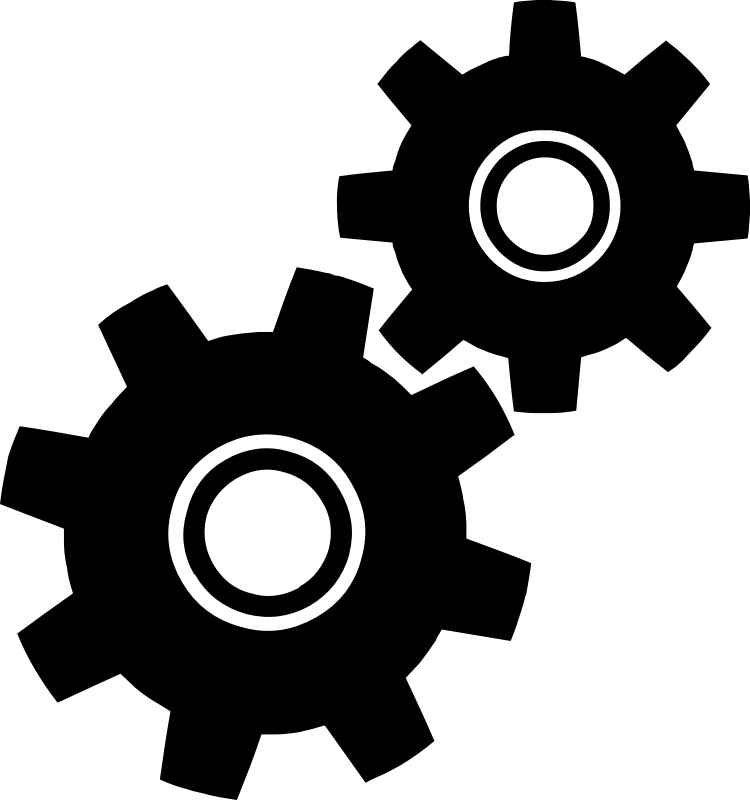
\includegraphics[width=\textwidth]{plots/gears.png}
    \end{figure}
  \column{0.6\textwidth}
  \begingroup
  \centering
    \fontsize{20pt}{22pt}\selectfont
    \vspace{1cm}
    \\
Machine learning is a branch of computer science and applied statistics covering algorithms that improves their performance at a given task based on sample data or experience.
  \endgroup
\end{columns}

\end{frame}

\begin{frame}{Data Science and Machine Learning}

\scriptsize

\begin{center}
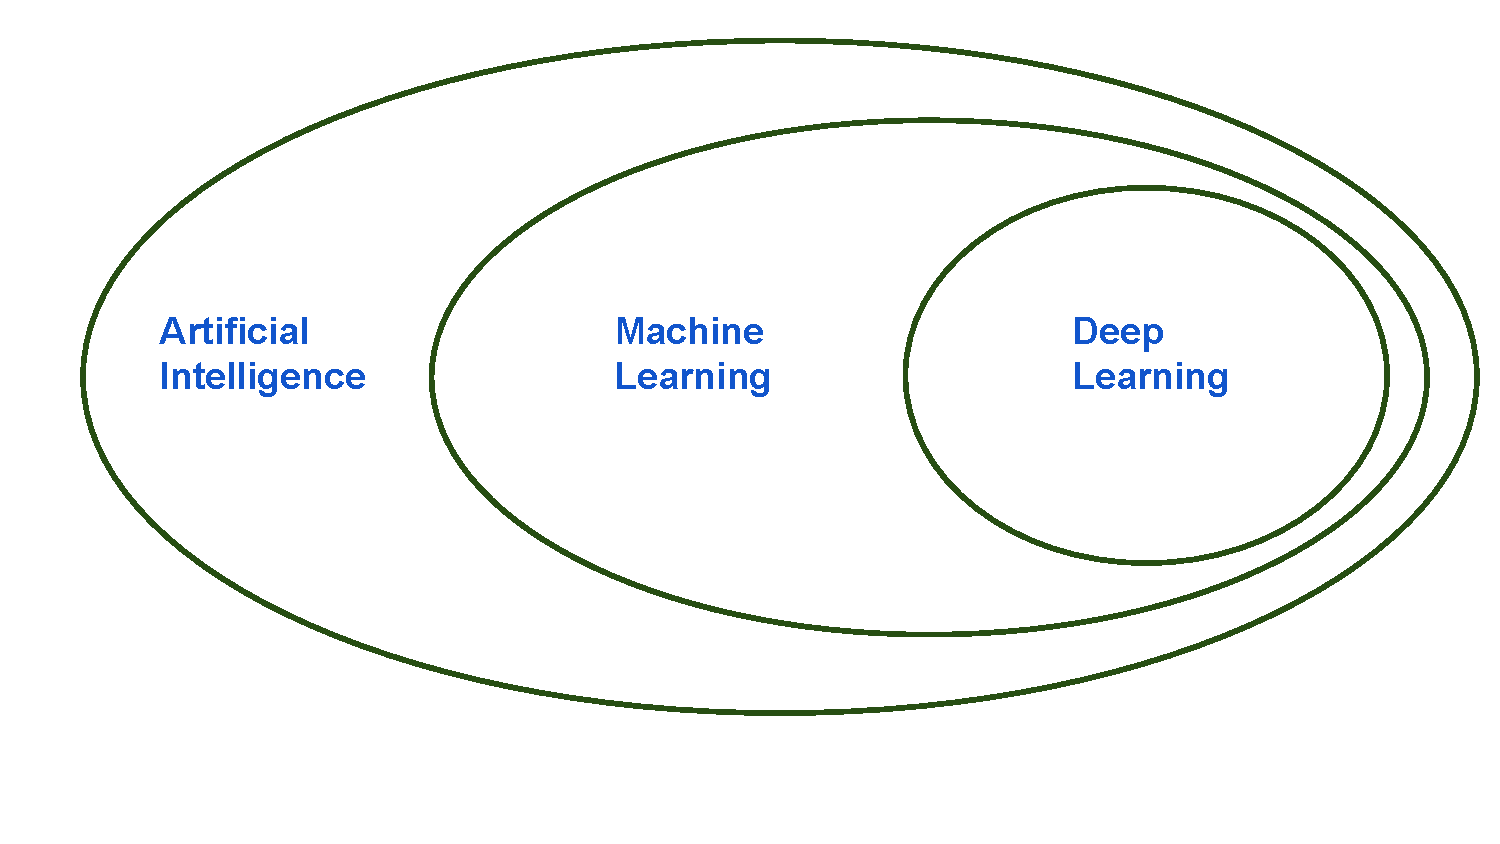
\includegraphics[width=0.95\textwidth]{plots/learning.pdf} 
\end{center}

\normalsize 

\end{frame}

%%%%%%%%%%%%%%%%%%%%%%%%%%%%%%%%%%%%%%%%%%%%%%%%%%

\section{Supervised Learning Scenario}

\begin{frame}{Data, Target and Input Features}
Imagine you want to investigate how salary and workplace conditions affect productivity of employees.

\scriptsize

\begin{center}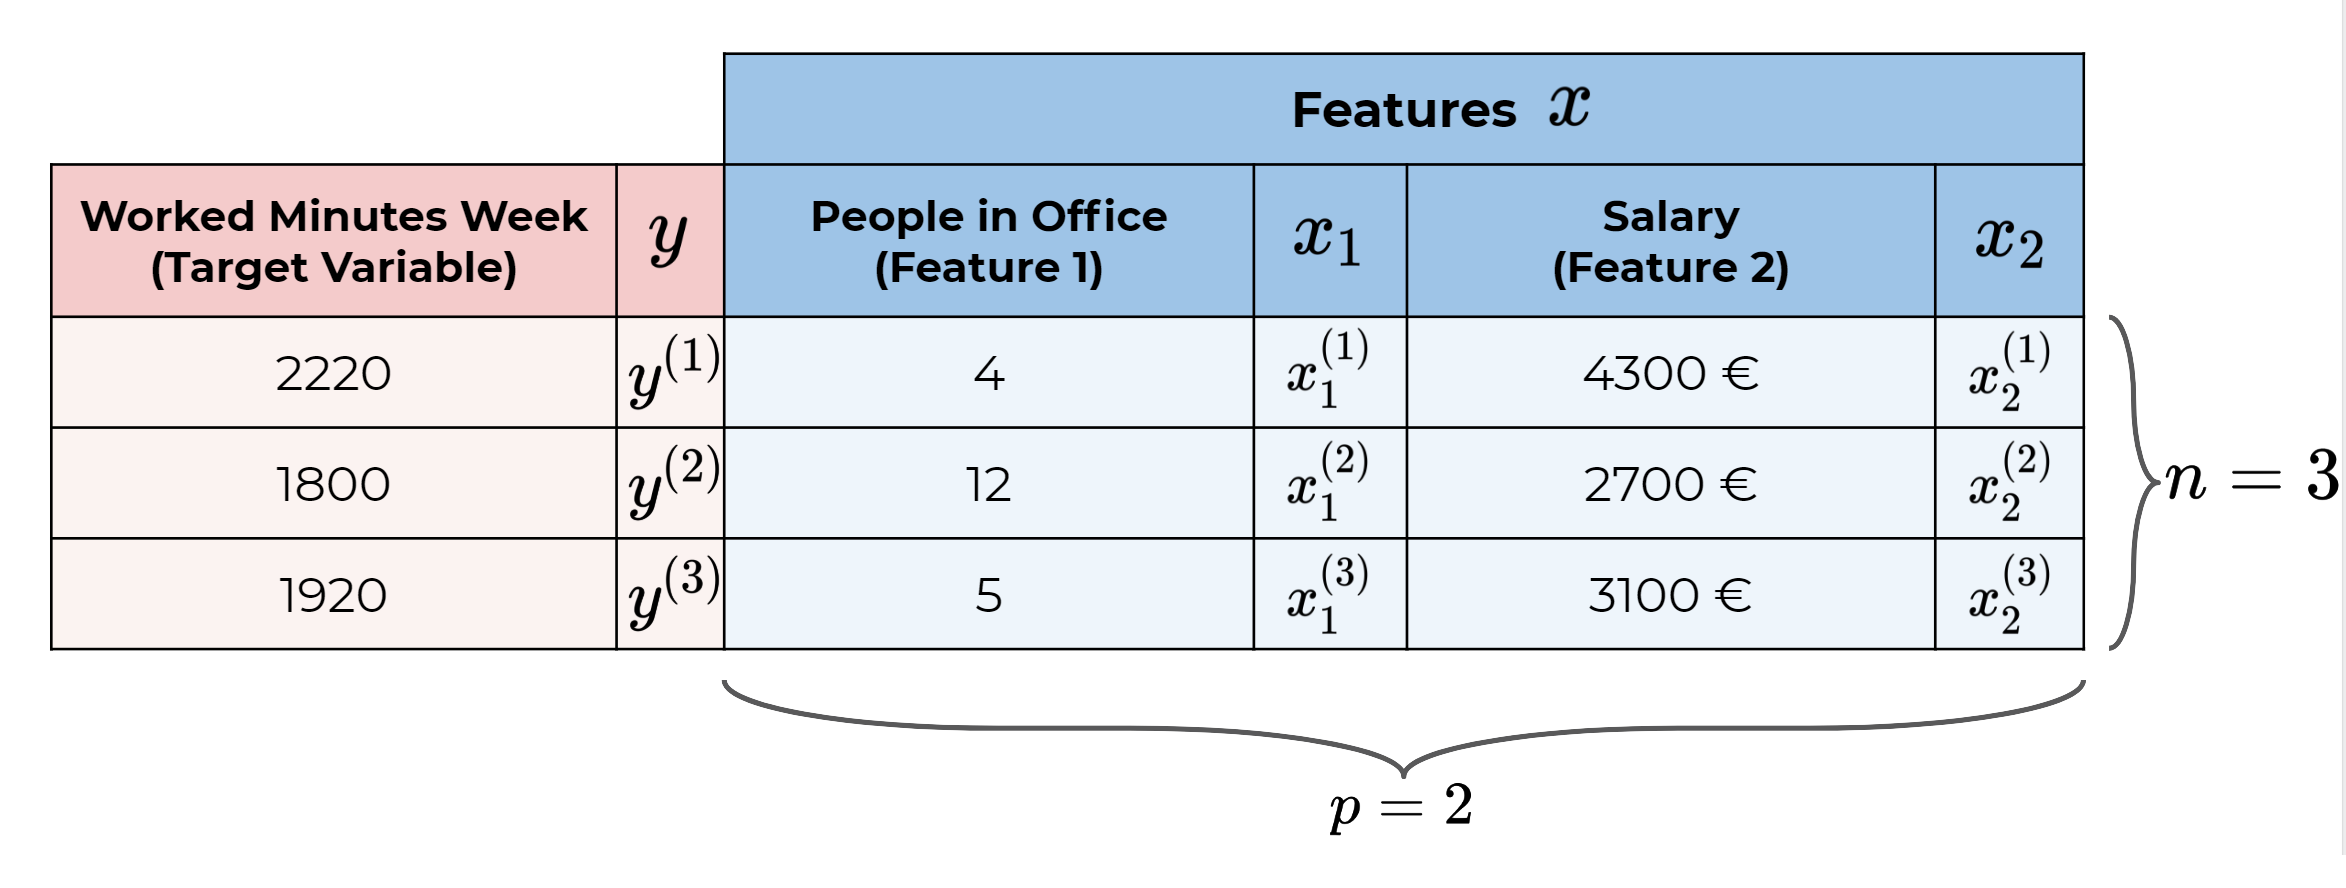
\includegraphics[width=0.8\textwidth]{plots/data_table} \end{center}

\normalsize 

\vspace{-0.5cm}

The whole data set is expressed by \[
\D = \Dset
\] with the \(i\)-th observation \(\xyi\) $\in \mathcal{X}x\mathcal{Y}$.

$\mathcal{X}$ is called input and $\mathcal{Y}$ output or target space.

\end{frame}


\begin{frame}{Target and Features Relationship}

\begin{itemize}

\item
  For our observed data we know which outcome is produced:
\end{itemize}

\vspace{-0.5cm}

\scriptsize

\begin{center}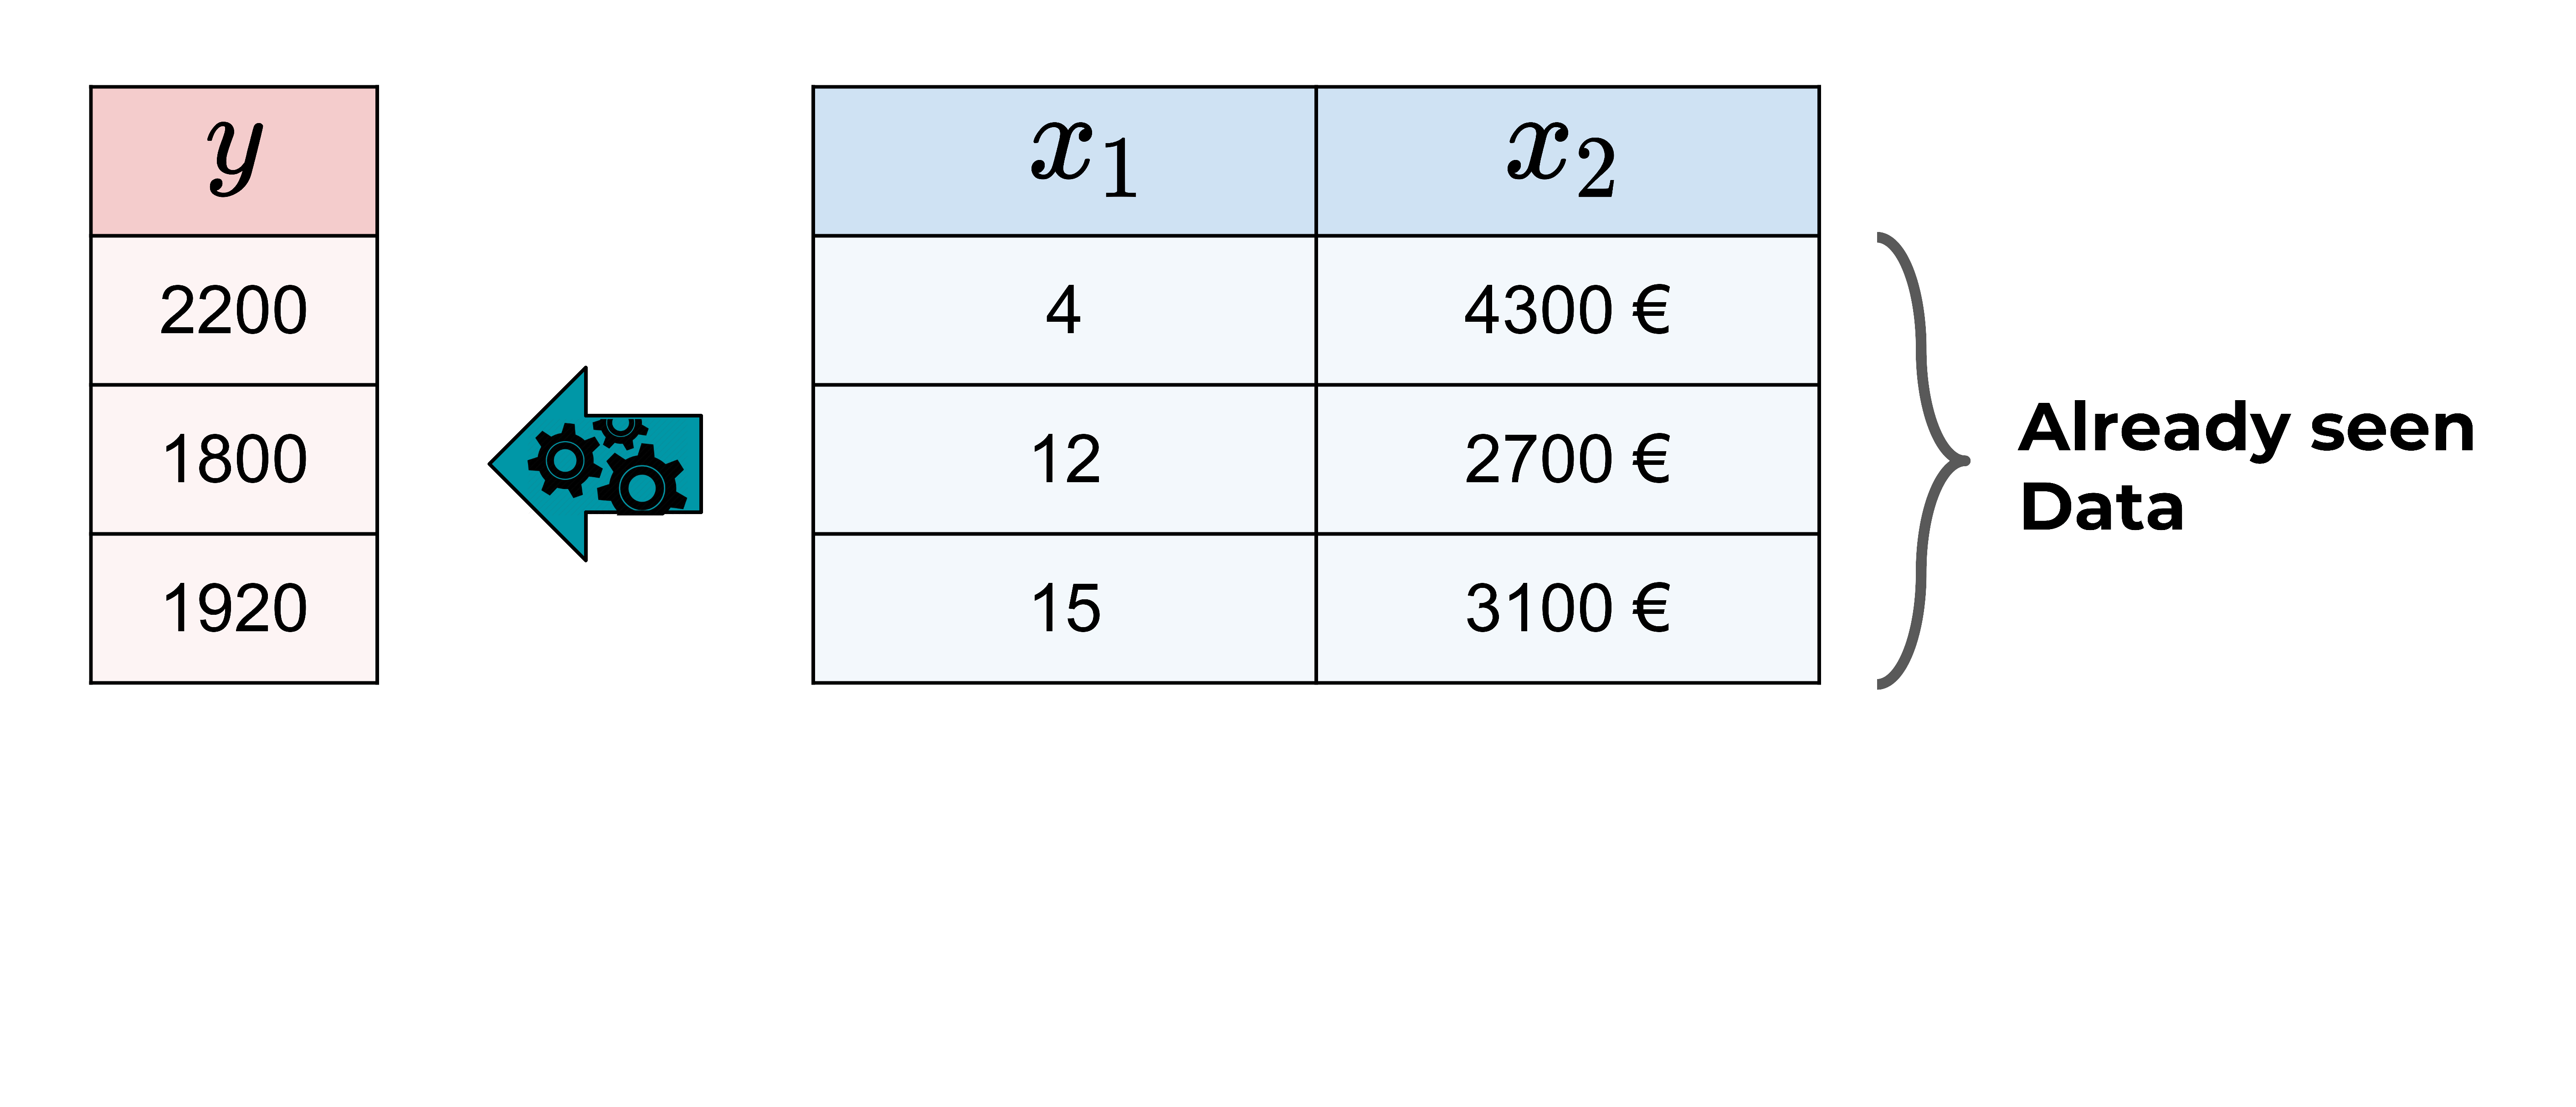
\includegraphics[width=0.9\textwidth]{plots/new_data0_web} \end{center}

\normalsize 

\end{frame}

\begin{frame}{Target and Features Relationship}

\begin{itemize}

\item
  For new employees we can just observe the features:
\end{itemize}

\vspace{-0.5cm}

\scriptsize

\begin{center}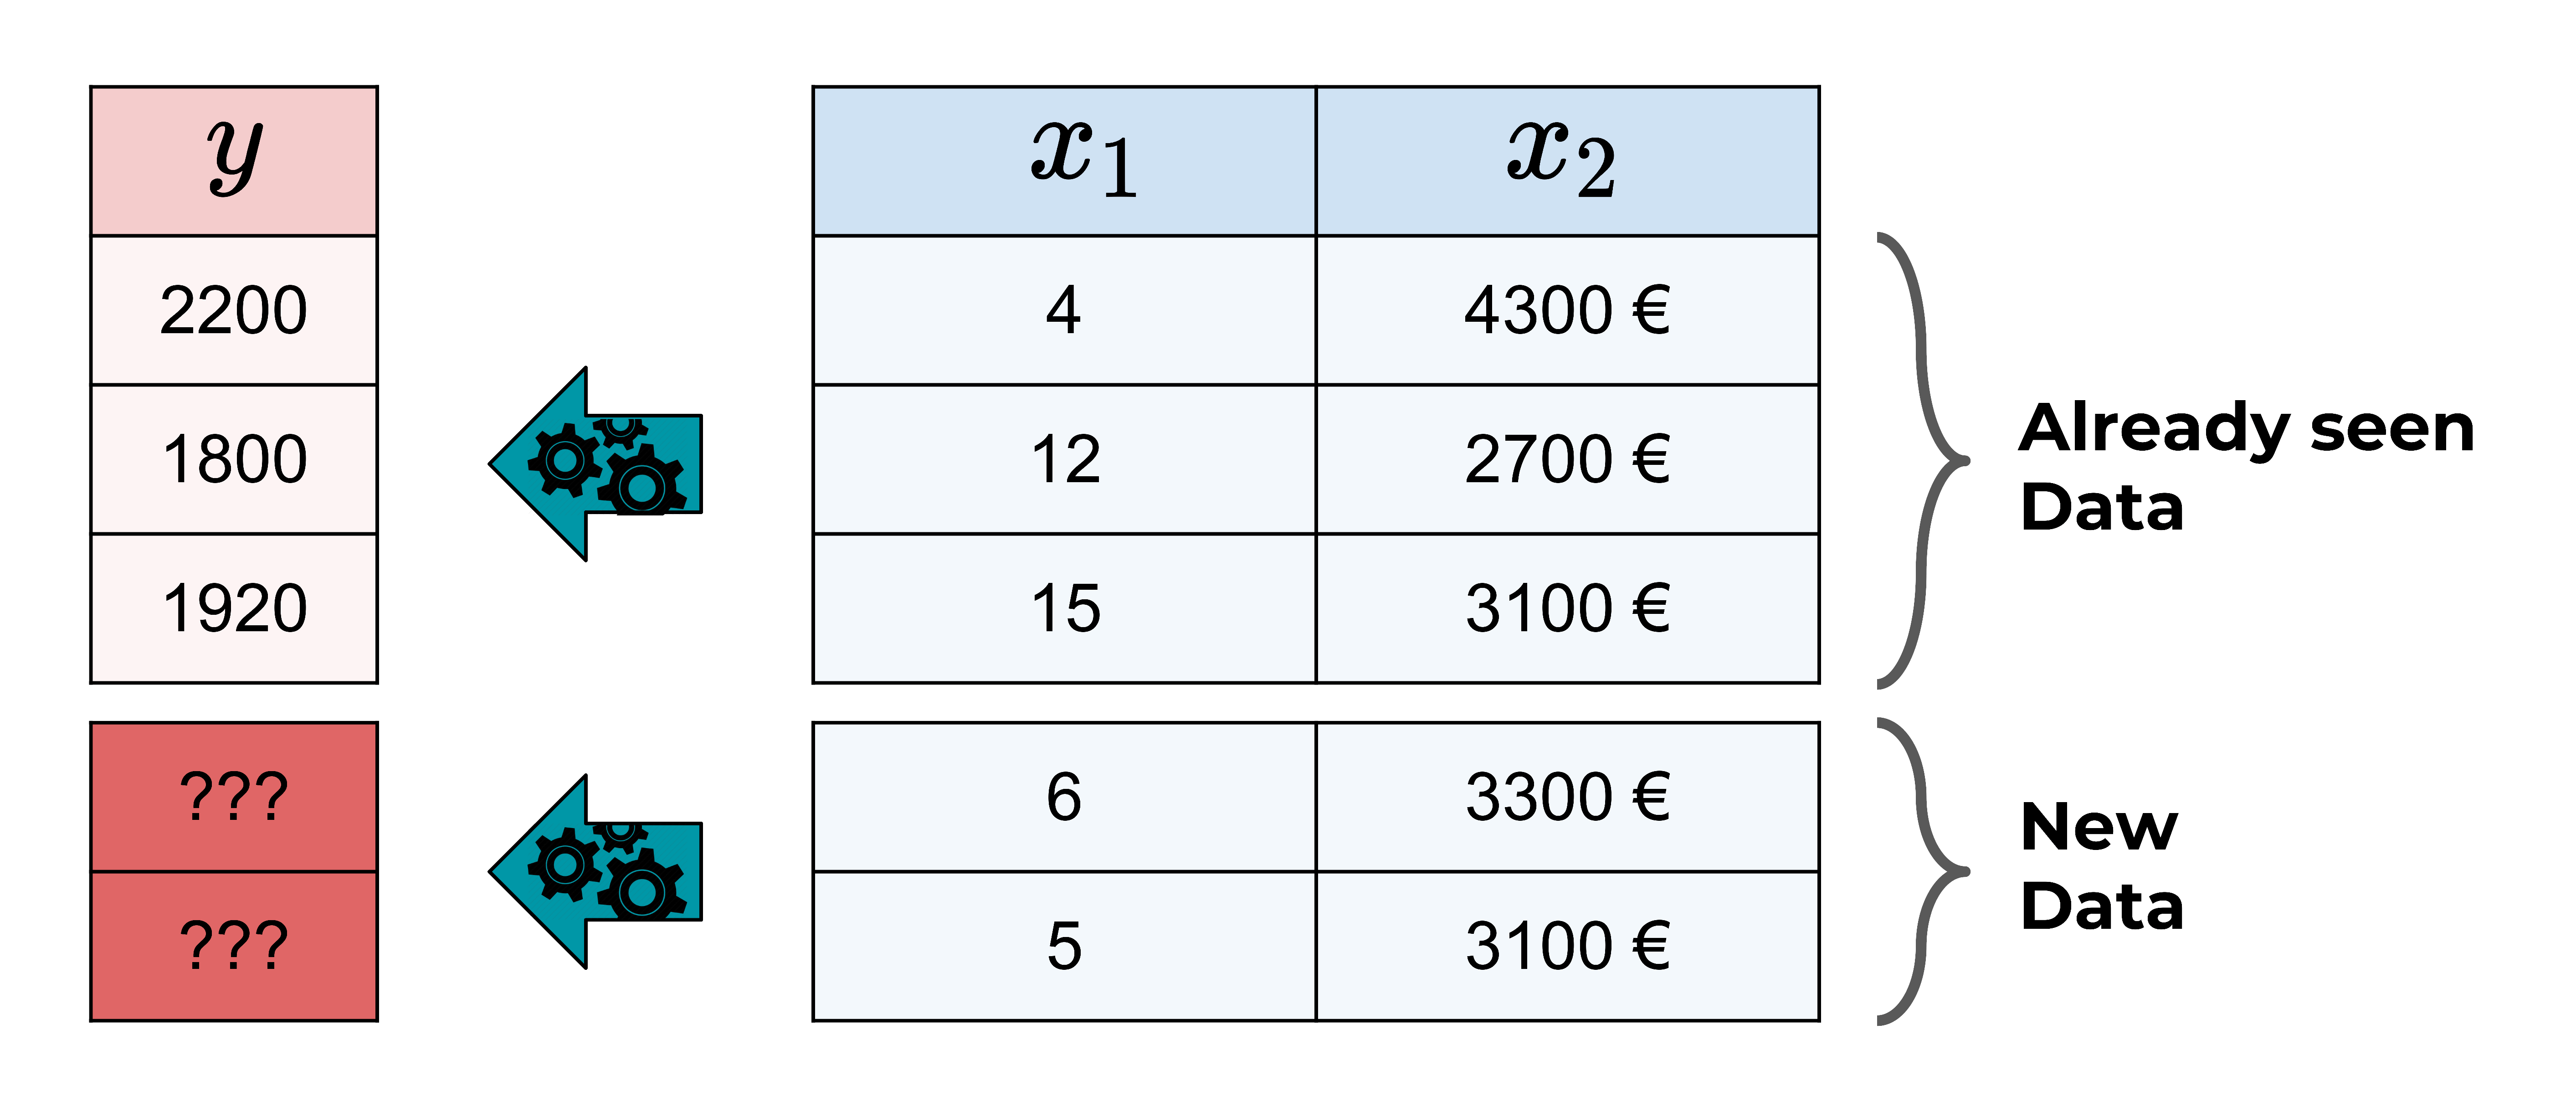
\includegraphics[width=0.9\textwidth]{plots/new_data1_web} \end{center}

\normalsize 

\vspace{-0.5cm}
\end{frame}


\begin{frame}{Target and Features Relationship}

\scriptsize

\begin{center}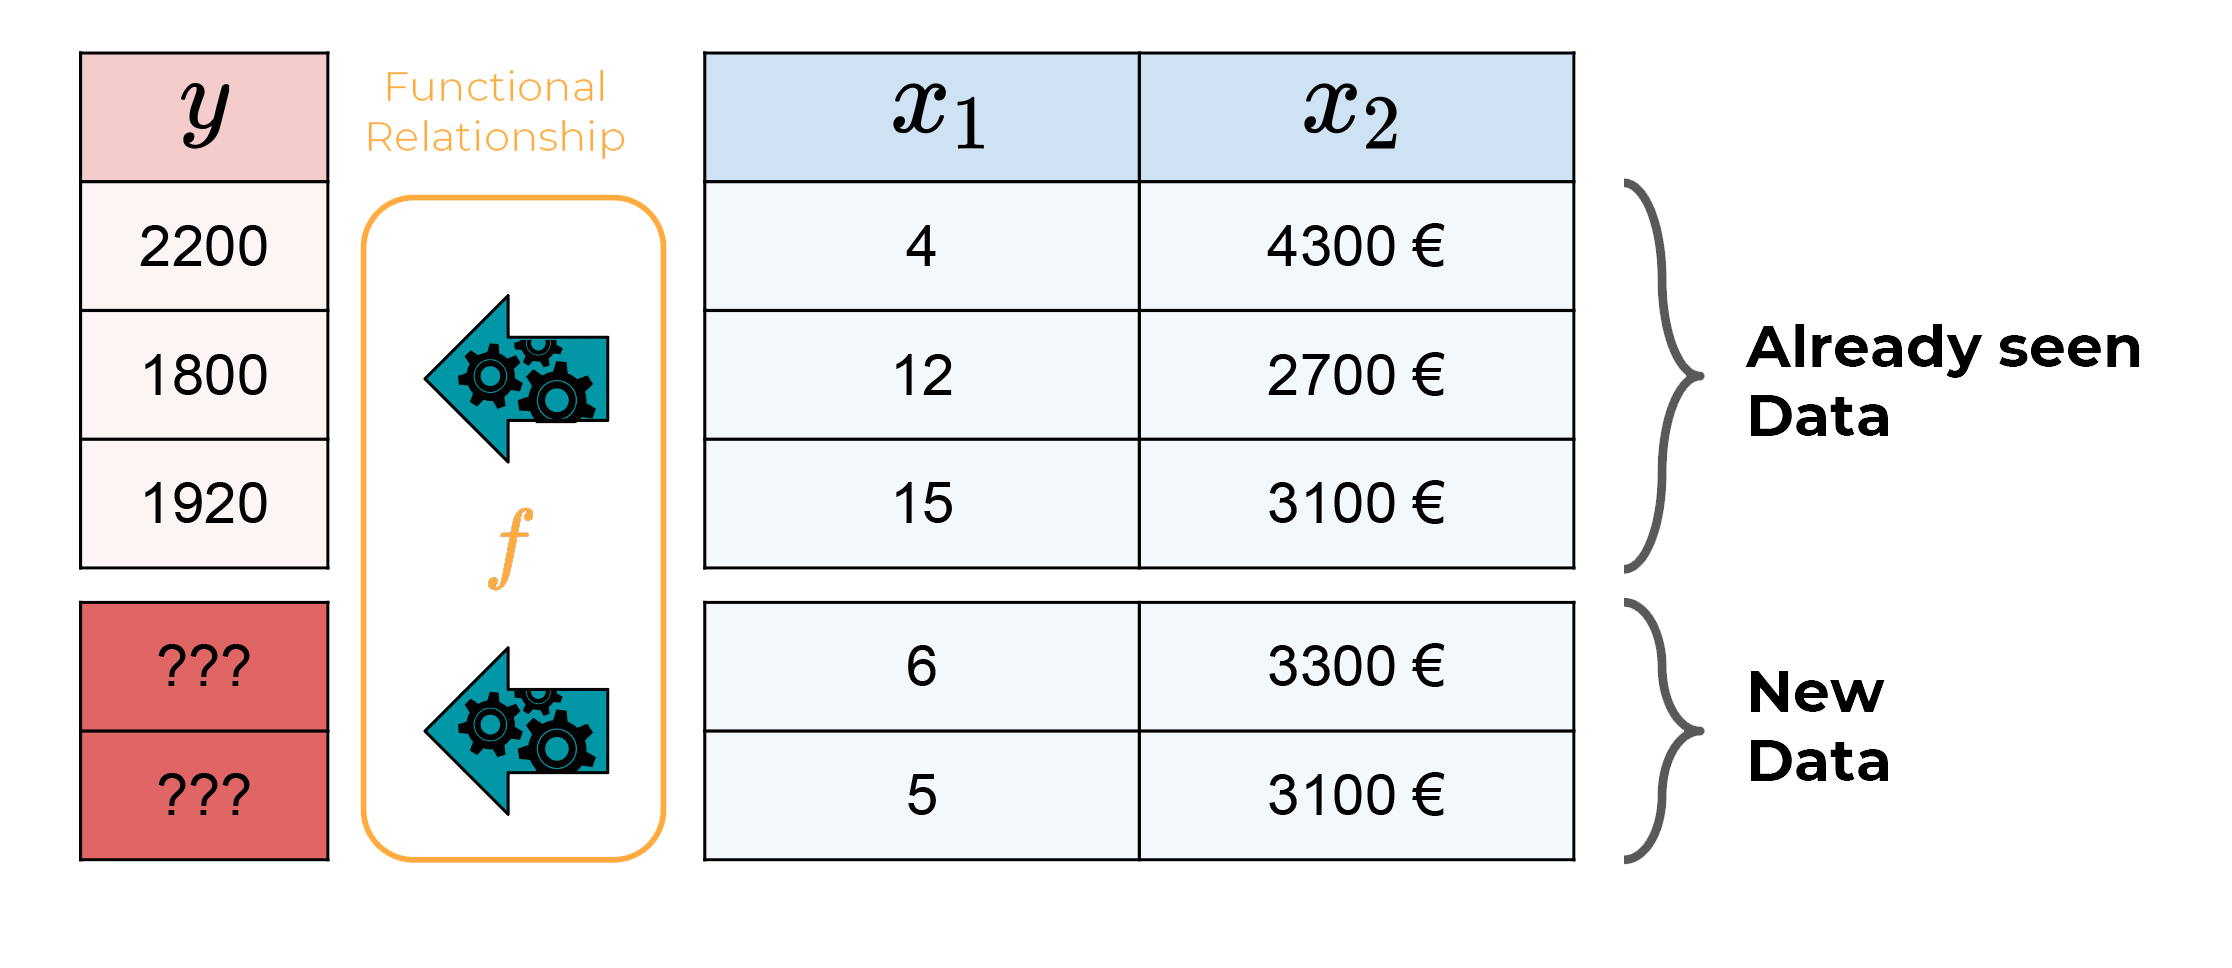
\includegraphics[width=\textwidth]{plots/what_is_a_model_web} \end{center}

\(\Rightarrow\) The goal is to predict the target variable for
\textbf{unseen new data} by using a \textbf{model} trained on the
already seen \textbf{train data}.

\normalsize 

\end{frame}

\begin{frame}{Target and Features Relationship}

\begin{itemize}
\item
  In ML, we want to be \enquote{lazy}. We do not want to specify \(f\)
  manually.
\item
  We want to learn it \textbf{automatically from labeled data}.
\item
  Later we will see that we do have to specify something, like \(f\)'s
  functional form and other stuff.
\item
  Mathematically, we face a problem of function approximation: search
  for an \(f\), such that, for all points in the training data and also
  all newly observed points

\begin{center}
  \begin{tikzpicture}[->,>=stealth',shorten >=1pt,auto,node distance=1cm,
      thick,main node/.style={circle,fill=blue!20,draw,font=\sffamily\Large\bfseries}]
    \node[punkt] (natur) {$f$};
    \node[left=of natur] (x) {x};
    \node[right=of natur] (y) {f(x)};
    \path[every node/.style={font=\sffamily\small}]
    (natur) edge node {} (y)
    (x) edge node  {} (natur)
    ;
  \end{tikzpicture}
\end{center}

  predicted outcomes are very close to real targets: $\fx \approx y$

\end{itemize}

\begin{itemize}

\item
  We call this \textbf{supervised learning}.
\end{itemize}

\end{frame}

\begin{frame}{Supervised Learning Task}

\begin{itemize}
\item \textbf{Regression}: Given an input $x$, predict corresponding output from $\mathcal{Y} \in \R^g, 1 \leq g < \infty$.
\item \textbf{Classification}: Assigning an input $x$ to one class of a finite set of classes $\Yspace = \{C_1,...,C_g\}, 2 \leq g < \infty$.
\item \textbf{Density estimation}: Given an input $x$, predict the probability distribution $p(y|x)$ on $\Yspace$.
\end{itemize}

\end{frame}

%%%%%%%%%%%%%%%%%%%%%%%%%%%%%%%%%%%%%%%%%%%

\begin{frame}{What is a Model?}

A \textbf{model} (or \textbf{hypothesis}) $f : \Xspace \rightarrow \Yspace$ maps inputs (or input features) to outputs (or targets).

A \textbf{hypothesis class} $H$ is a set of such functions.

\scriptsize

\begin{center}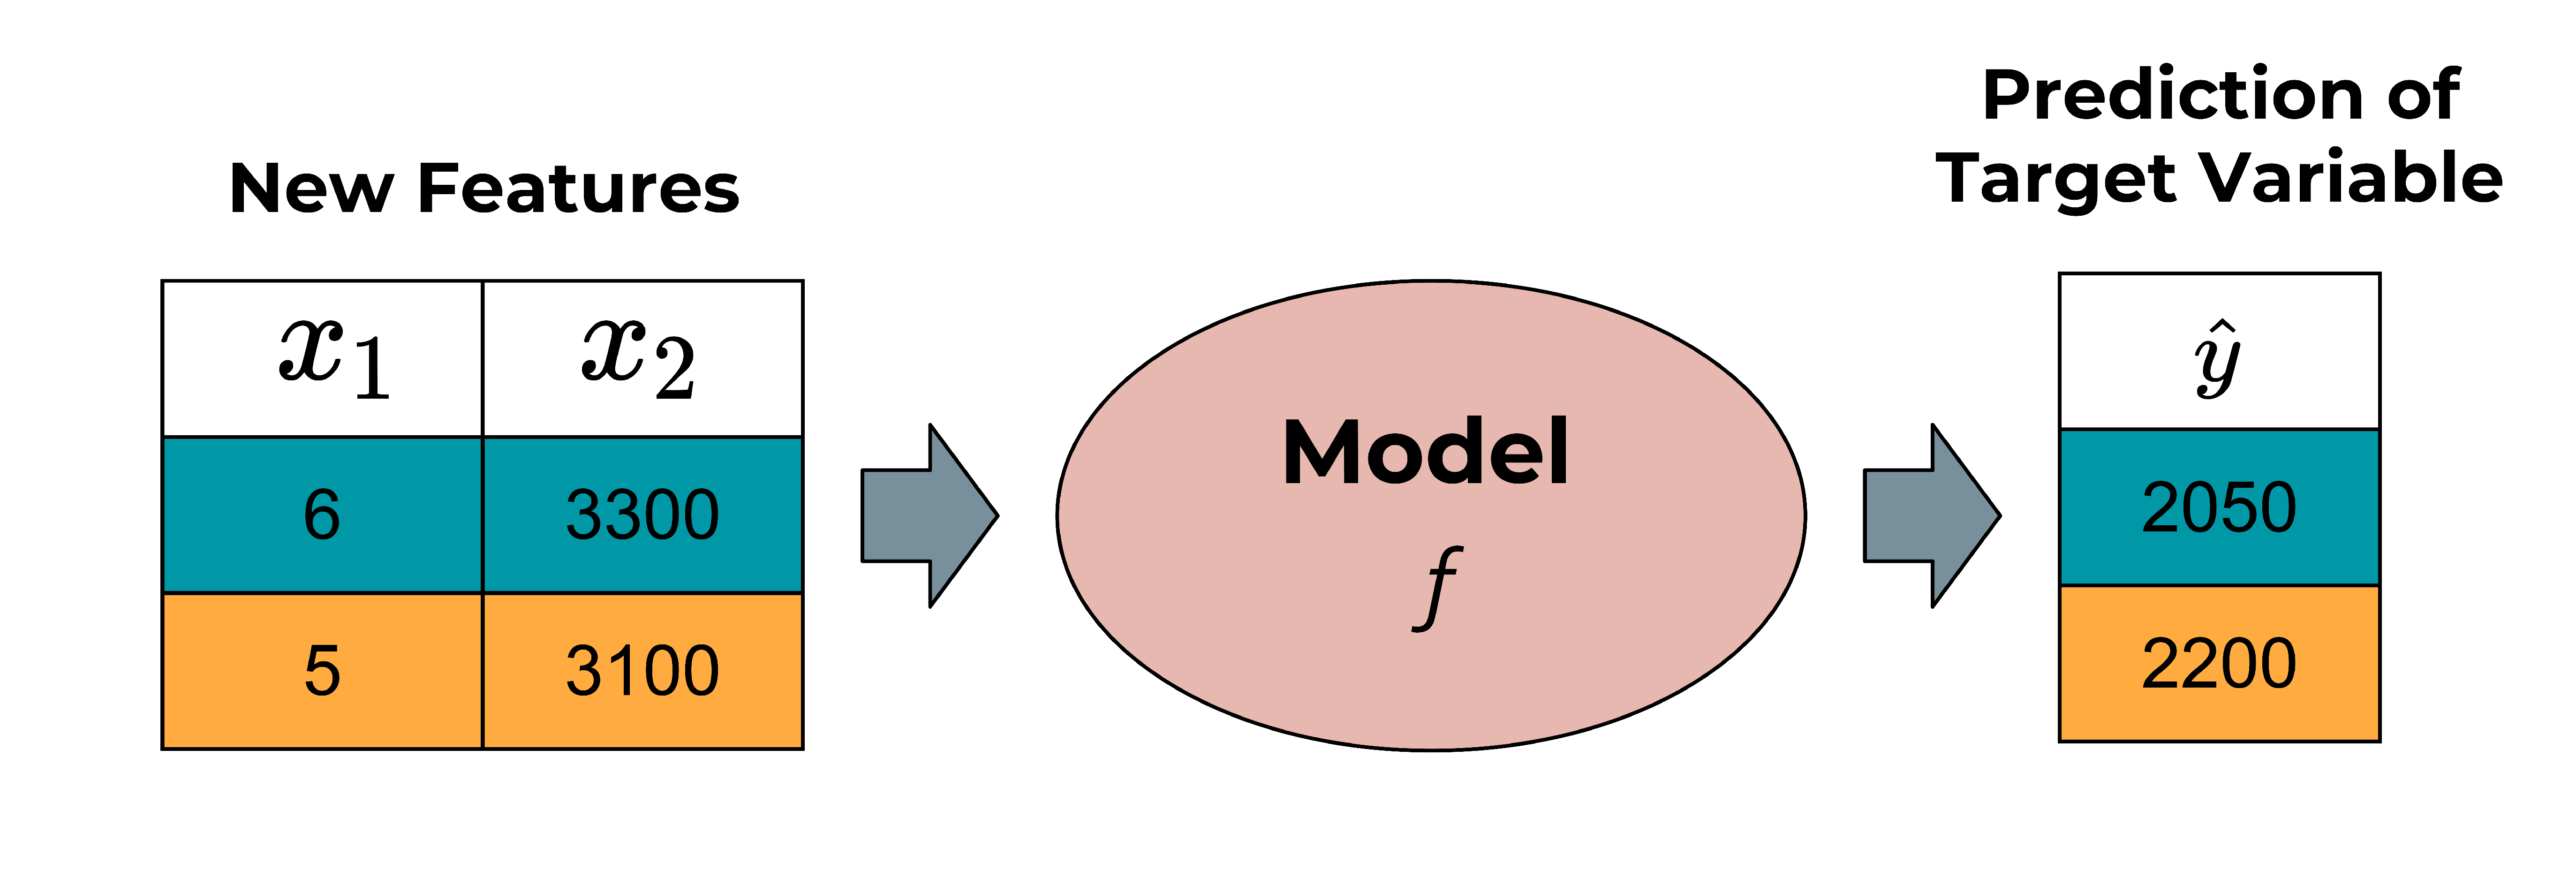
\includegraphics[width=0.9\textwidth]{plots/the_model_web} \end{center}

\normalsize 

\end{frame}

\begin{frame}{What is a Learner?}

The \textbf{learner} (inducer, \textbf{learning algorithm}) takes our labeled data set
(\textbf{training set}) and produces a model (which again is a
function):

Applying a learning algorithm means coming up with a hypothesis given sample data. 
Formally, it maps:
$$\{((x^{(1)},y^{(1)}),...,(x^{(n)},y^{(n)}))\} \subset \Xspace \times \Yspace \rightarrow \Hspace$$

\vspace{-0.5cm}

\scriptsize

\begin{center}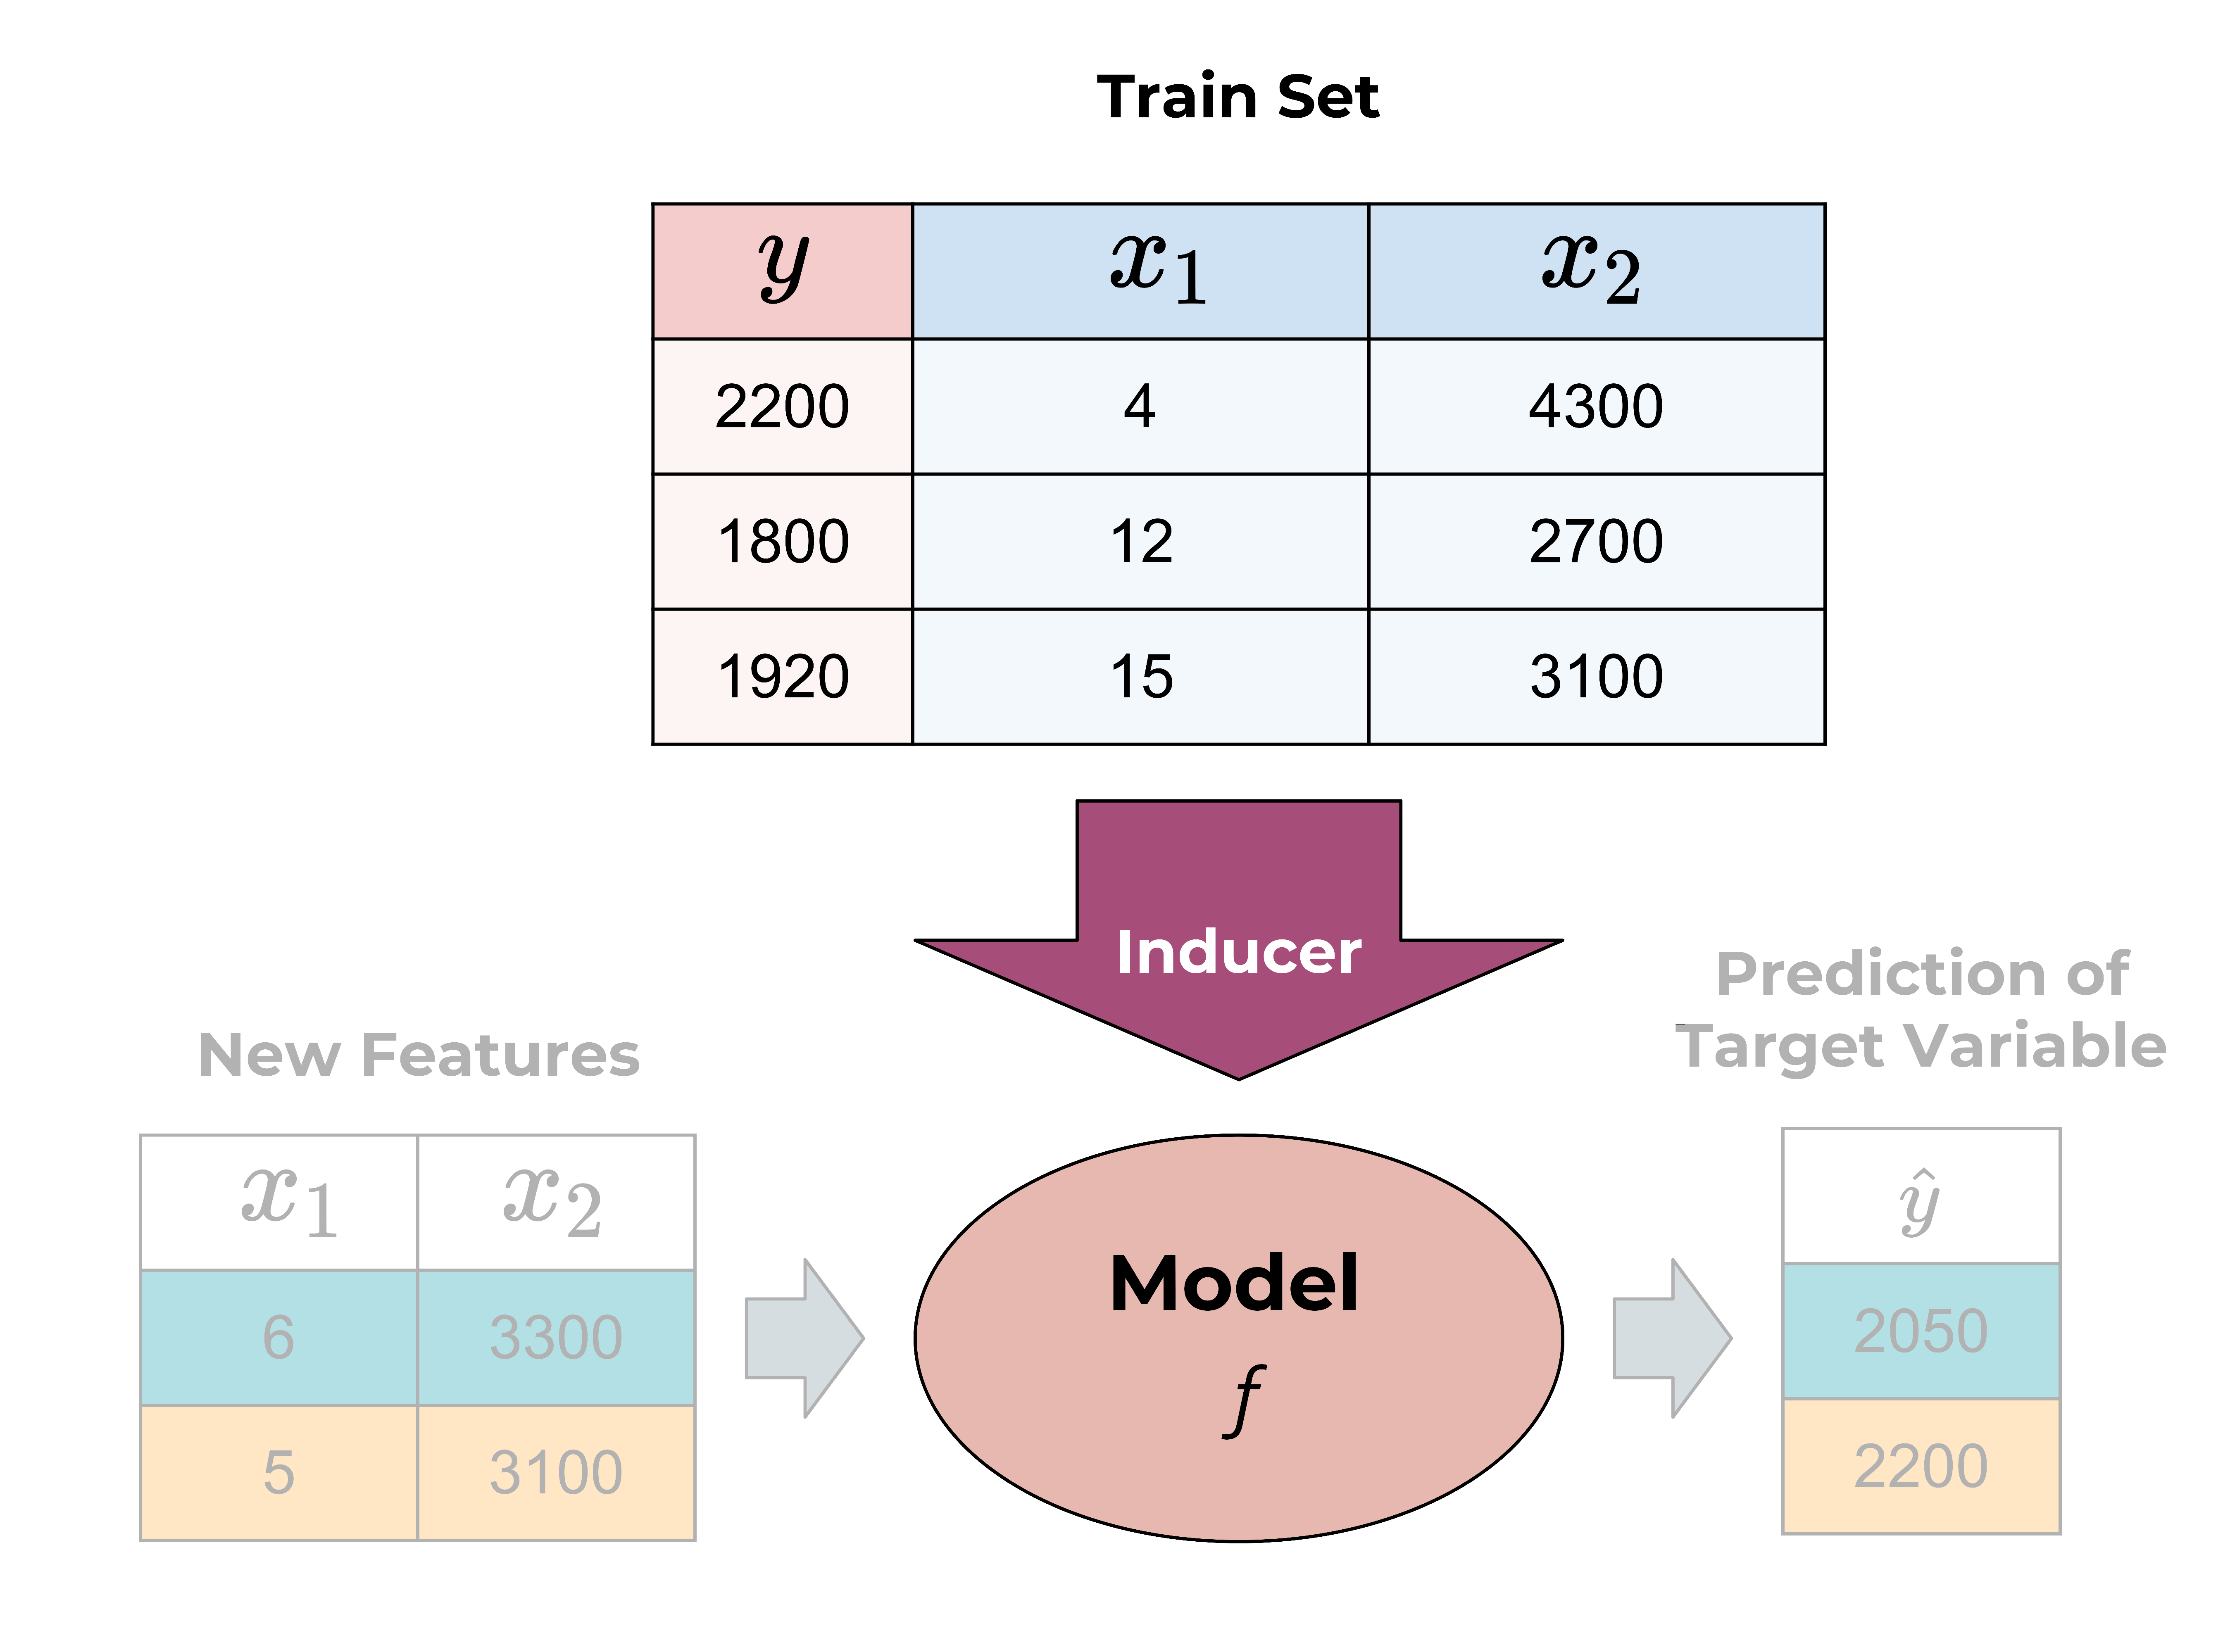
\includegraphics[width=0.7\textwidth]{plots/the_inducer_web} \end{center}

\normalsize 

\end{frame}

\begin{frame}{How to Evaluate Models}

\begin{itemize}

\item
  Simply compare predictions from model with truth:
\end{itemize}

\scriptsize

\begin{center}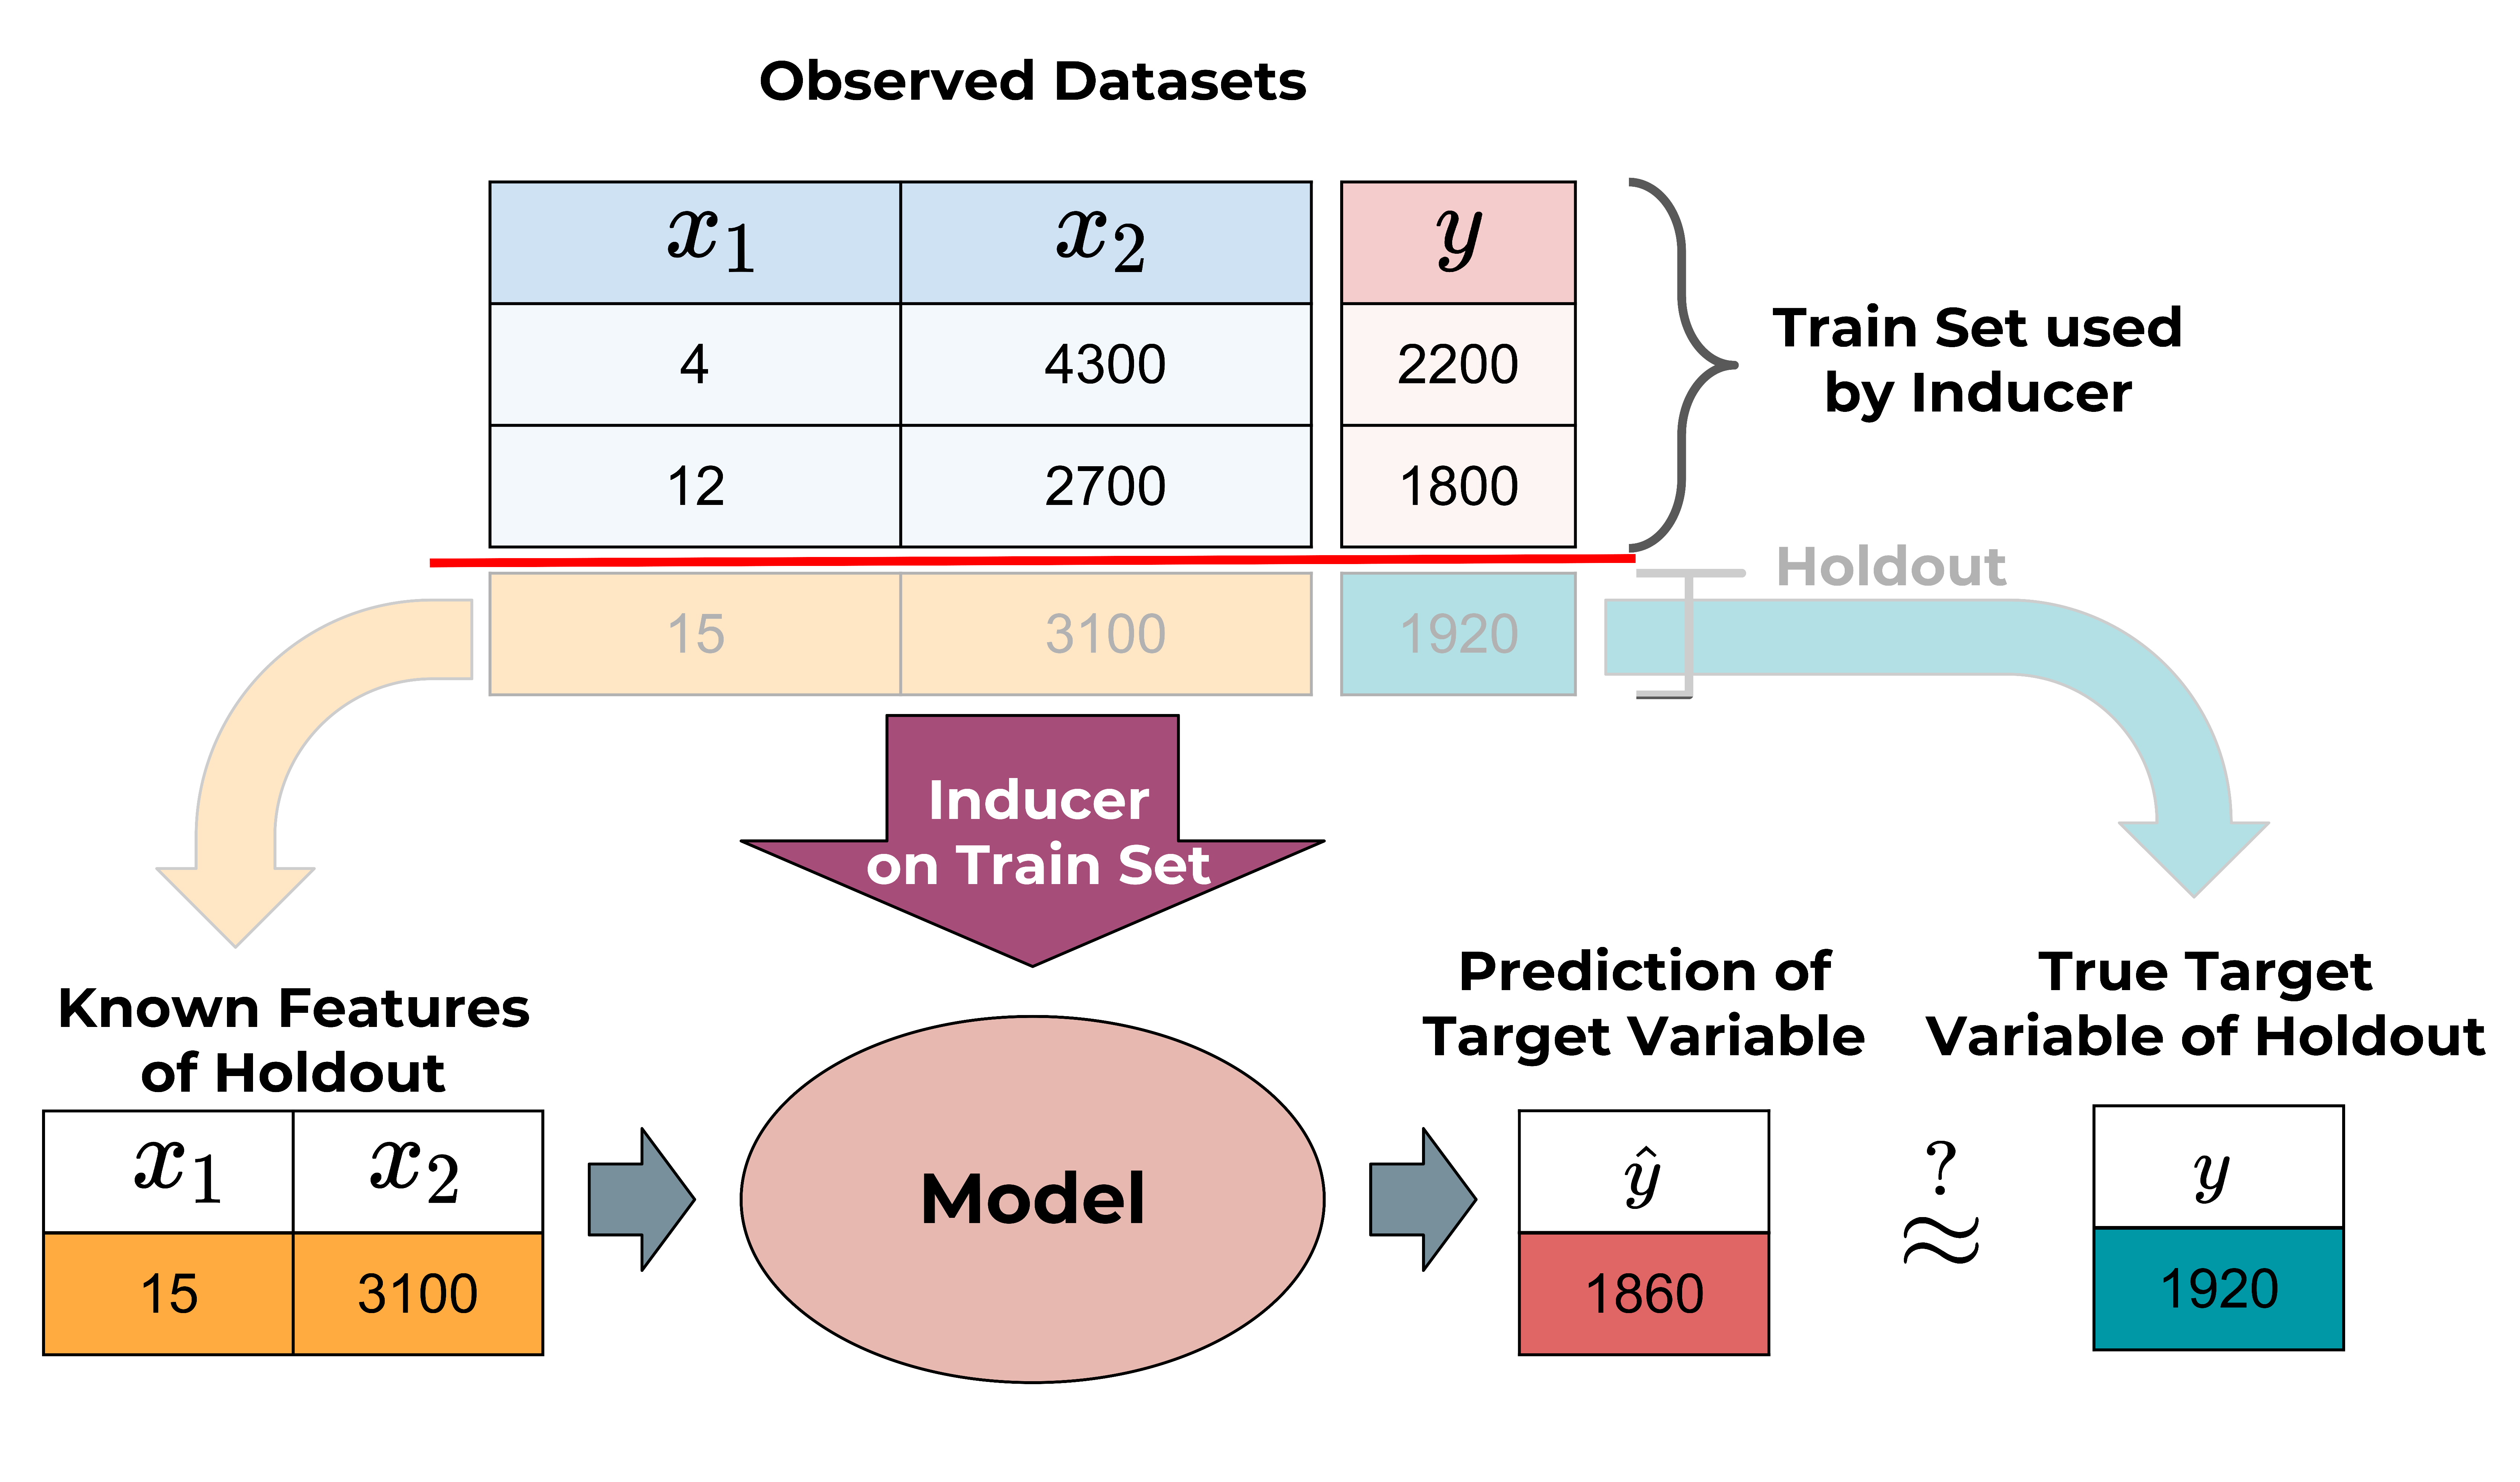
\includegraphics[width=0.8\textwidth]{plots/eval_inducer1_web} \end{center}

\normalsize 
\end{frame}

\begin{frame}{Learner Decomposition}

Nearly all ML supervised learning training algorithms can be described
by three components:

\begin{center}
  \textbf{Learning = Hypothesis Space + Evaluation + Optimization}
\end{center}

\begin{itemize}
\item
  \textbf{Hypothesis Space:} Defines functional
  structures of \(f\) we can learn.
\item
  \textbf{Evaluation:} How well does a certain hypothesis score on a
  given data set? Allows us to choose better candidates over worse ones.
\item
  \textbf{Optimization:} How do we search the hypothesis space? Guided
  by the evaluation metric.
\item
  All of these components represent important choices in ML which can
  have drastic effects:
  \newline
  If we make smart choices here, we can tailor our learner to our needs
  - but that usually requires quite a lot of experience and deeper
  insights into ML.
\end{itemize}

\end{frame}

%%%%%%%%%%%%%%%%%%%%%%%%%%%%%%%%%%%%%%%

\begin{vbframe}{Risk and loss function}

Let \(\mathbb P_{xy}\) be the joint distribution of \(x\) and \(y\), where $\D$ is i.i.d sampled from. It defines all aspects of the generating process where our data comes from. 
\vfill
The quality of the prediction $y=\fx$ of a model is measured by a \textbf{loss function} $\Lxy $.
\vfill
This is a  function $L :\Yspace \times \Yspace \rightarrow [0, \infty[$ with the property $L(y, y) = 0$ for $y \in  \Yspace$.
\vfill
E.g. the squared error $\Lxy = (y-\fx)^2$,
\vfill
Its expectation w.r.t. $\Pxy$ is the so-called \textbf{risk},
  $$ \riskf = \E [\Lxy] = \int \Lxy d\Pxy. $$
\end{vbframe}

%%%%%%%%%%%%%%%%%%%%%%%%%%%%%%%%

\begin{frame}{empirical risk minimization}
Obvious aim: Minimize $\riskf$ over $f$.
 
Usually  $\P_{xy}$ is unknown, but we can approximate $\riskf= \E [\Lxy]$ based on
the data $\D$, by means of the \textbf{empirical risk}

$$
\riske(f) = \frac{1}{n} \sumin \Lxyi
$$

Learning then amounts to \textbf{empirical risk minimization}
$$
\fh = \argmin_{f \in \Hspace} \riske(f).
$$

\end{frame}

%%%%%%%%%%%%%%%%%%%%%%%%%%%%%%%%%%%%%%%%%%%%%%%%%%%%%%%%%
\begin{frame}{empirical risk minimization}

When $f$ is parameterized by $\theta$, this becomes:

\begin{eqnarray*}
\riske(\theta) & = & \frac{1}{n} \sumin \Lxyit \cr
\hat{\theta} & = & \argmin_{\theta \in \Theta} \riske(\theta)
\end{eqnarray*}


\begin{itemize}
\item Learning (often) means solving the above \emph{optimization problem}, which implies a tight connection between ML and optimization.

\item Note that (with a slight abuse of notation), if it is more convenient, and as there is no difference w.r.t.
the minimizer, we might also define the $\riske$ 
as:

$$
\risket = \sumin \Lxyit
$$

\end{itemize}

\end{frame}

%%%%%%%%%%%%%%%%%%%%%%%%%%%%%%%%%%%%%%%%%%%%%%%%%%%%%

\section{(Linear) Regression}

\begin{frame}{Regression task}

\begin{itemize}
\item Given $\D = \Dset \subset \mathcal{X}x\mathcal{Y}$, where $\mathcal{X}\subseteq \R^p$ and $\mathcal{Y}\subseteq \R^g$
\item
  \textbf{Goal}: Learn $f:\mathcal{X} \rightarrow \mathcal{Y} $
\end{itemize}

\begin{center}
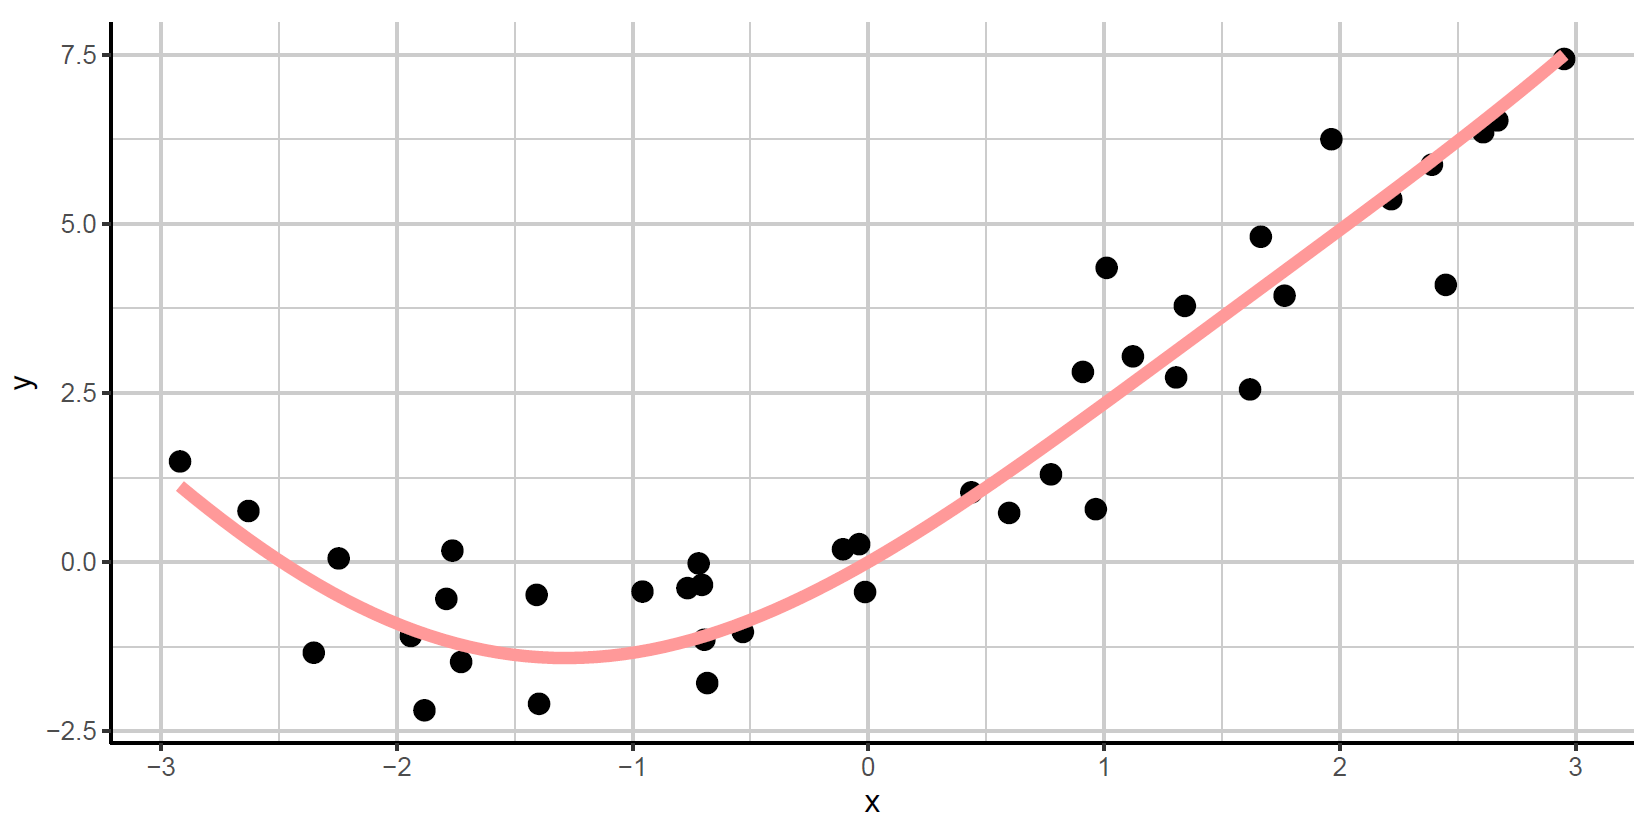
\includegraphics[width=0.8\textwidth]{plots/Reg-task.png}
\end{center}

\end{frame}

%%%%%%%%%%%%%%%%%%%%%%%%%%%%%%%%%%%%%%%%%%%%%%%%%%%%


\begin{frame}{straight line / uinvariate linear model}

\scriptsize

\begin{center}
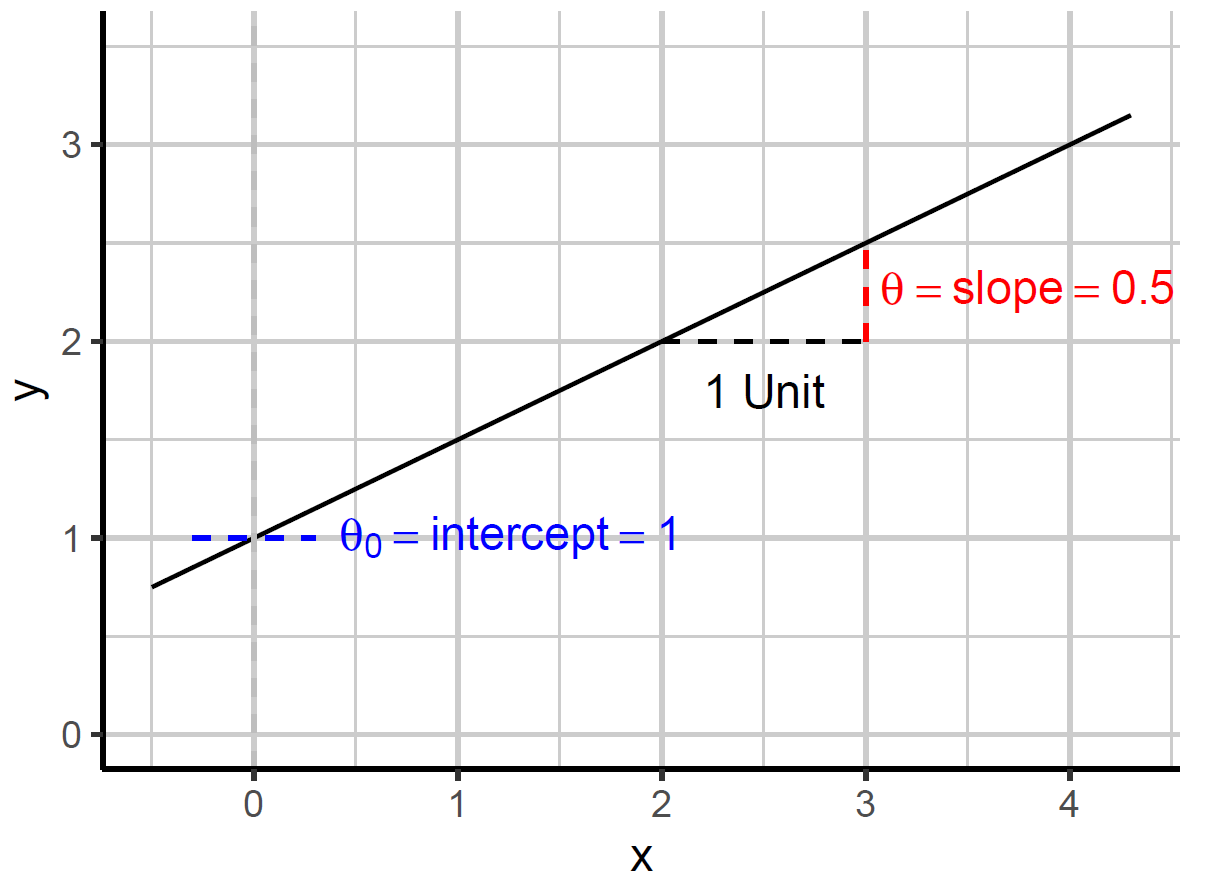
\includegraphics[width=0.7\textwidth]{plots/straight-line.png}
\end{center}


\normalsize 

\[
y = \theta_0 + \theta \cdot x
\]

\end{frame}

%%%%%%%%%%%%%%%%%%%%%%%%%%%%%%%%%%%%%%%%%%%%%%%%%%%%%

\begin{frame}{Linear Regression: Hypothesis Space}

\begin{itemize}
\item We want to learn a numerical target variable, by a linear transformation
of the features. So with \(\theta \in \mathbb{R}^p\) this mapping can be
written: \[
y = \fx = \theta_0 + \theta^T x
\]

\item This restricts the hypothesis space \(H\) to all linear functions in
\(\theta\): \[
H = \{ \theta_0 + \theta^T x\ |\ (\theta_0, \theta) \in \mathbb{R}^{p+1} \}
\]

\item Learning (or parameter estimation) now corresponds to finding  \((\theta, \theta_0\)), 
given observed labeled data \(\D\). 

\item We assume from now on that \(\theta_0\) is included in
\(\theta\) and write $f(x|\theta)$ to make the parameter dependency explicit. 
\end{itemize}

\end{frame}

%%%%%%%%%%%%%%%%%%%%%%%%%%%%%%%%%%%%%%%%%%%%%%%%%%%%%%%%

\begin{frame}{Linear Regression: Evaluation}

We now measure training error as sum-of-squared errors (SSE). This is also
called the L2 loss, or L2 risk: \[
\risket = \operatorname{SSE}(\theta) = \sumin \Lxyit = \sumin \left(\yi - \theta^T \xi\right)^2
\]

\scriptsize

\begin{center}
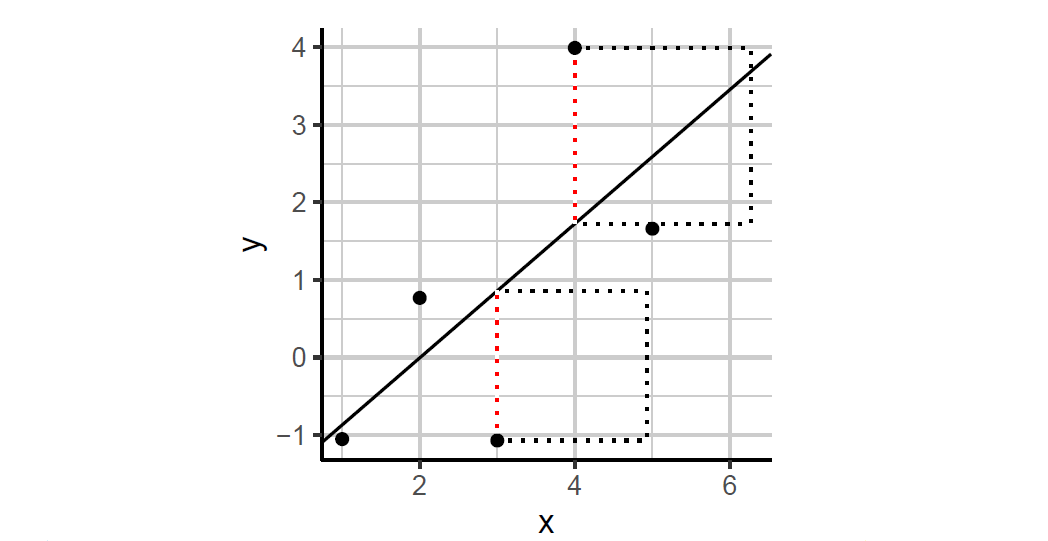
\includegraphics[width=0.6\textwidth]{plots/lin-reg.png}
\end{center}


\normalsize  \vspace{-0.4cm} Optimizing the squared error is
computationally much simpler than optimizing the absolute differences
(this would be called L1 loss).

\end{frame}


\begin{frame}{Linear Regression: Optimization}

We want to find the parameters of the LM / an element of the hypothesis
space H that best suits the data. So we evaluate different candidates
for \(\theta\).

\begin{itemize}
\item
  A first (random) try yields an SSE of 20.33 (\textbf{Evaluation}).
\end{itemize}

\begin{center}
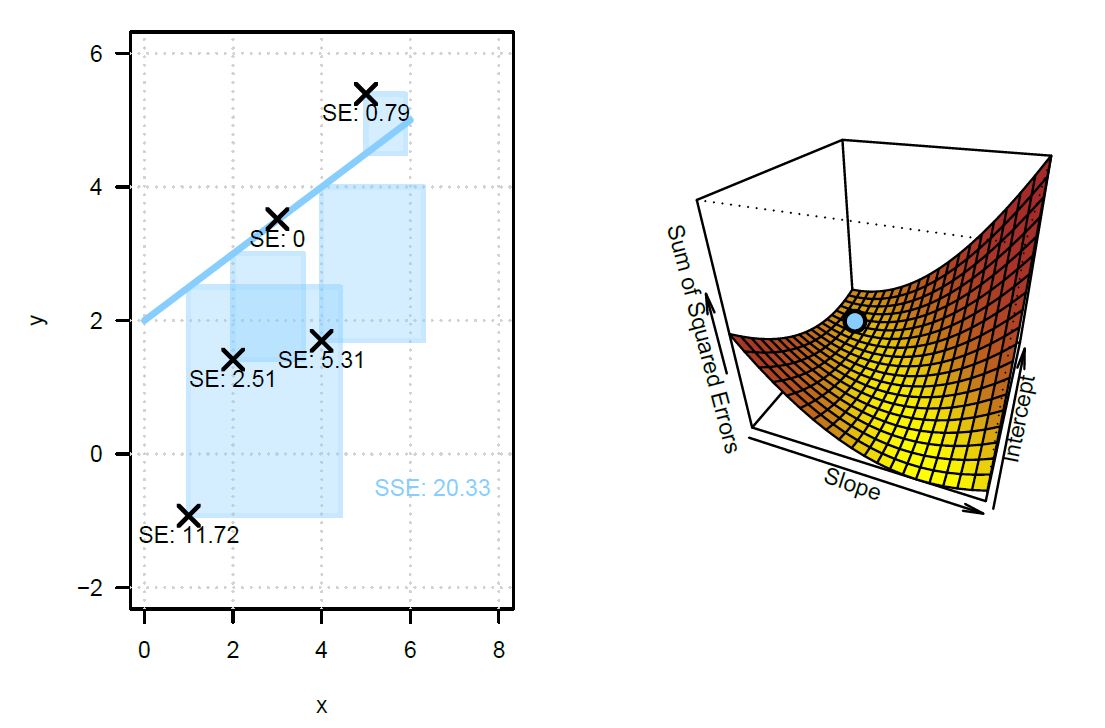
\includegraphics[width=0.6\textwidth]{plots/lin-reg-optim01.png}
\end{center}


\end{frame}


\begin{frame}{Linear Regression: Optimization}

We want to find the parameters of the LM / an element of the hypothesis
space H that best suits the data. So we evaluate different candidates
for \(\theta\).

\begin{itemize}
\item
  Another line yields an lower SSE of 18.51 (\textbf{Evaluation}).
\end{itemize}

\begin{center}
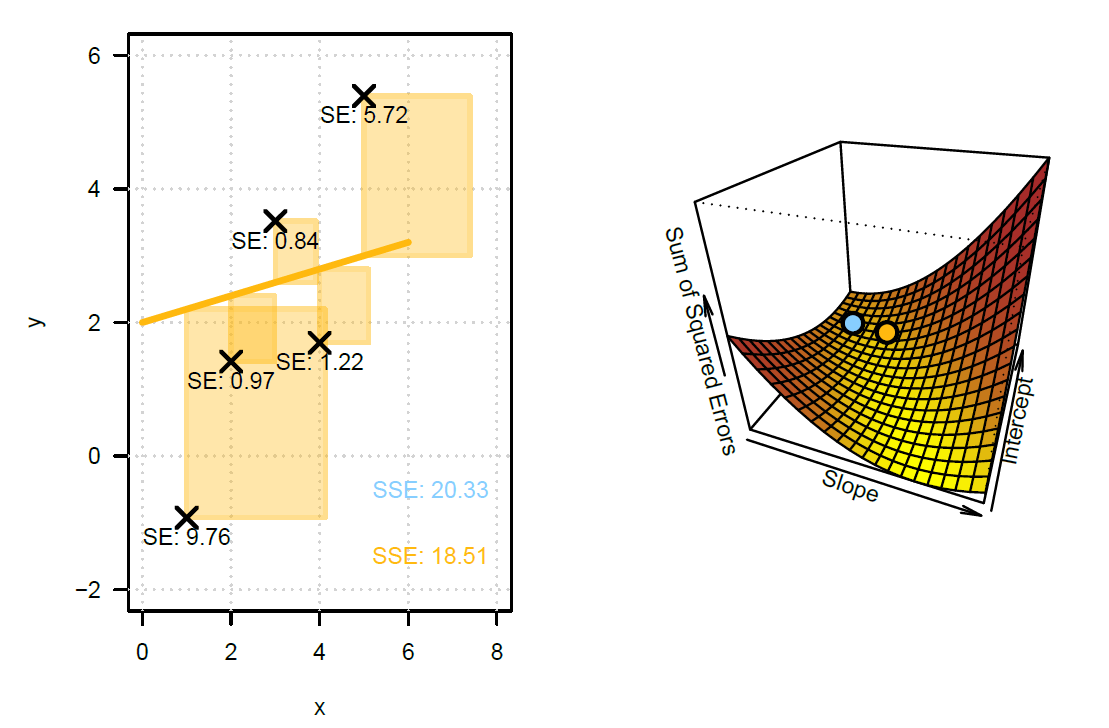
\includegraphics[width=0.6\textwidth]{plots/lin-reg-optim02.png}
\end{center}

\end{frame}

%%%%%%%%%%%%%%%%%%%%%%%%%%%%%%%%%%%%%%%%%%%%%%%%%%%%

\begin{frame}{Linear Regression: Optimization}

\begin{itemize}

\item Instead of guessing parameters we can find the optimal value analytically: \[
\hat{\theta} = \argmin_{\theta} \risket = \argmin_{\theta} \|y - X\theta\|^2_2
\]  where \(X\) is the \(n \times (p+1)\)-feature-data-matrix, also called
\emph{design matrix}.

\item Differentiating $\risket $ w.r.t $\theta$  and setting the derivative to zero
\[\frac{\delta}{\delta\theta} \risket = 0
 \qquad \Rightarrow\ 
 X^T(y - X\theta) = 0\]
 yields the so-called \emph{normal equations}:
 $$
\thetah = (X^T X)^{-1} X^T y
$$

\end{itemize}

\end{frame}

%%%%%%%%%%%%%%%%%%%%%%%%%%%%%%%%%%%%%%%%%%%%%%%%%%%%%

\begin{vbframe}{Linear Regression: Optimization}

The optimal line has an SSE of 9.77 (\textbf{Evaluation})

\vspace{0.3cm}
\begin{center}
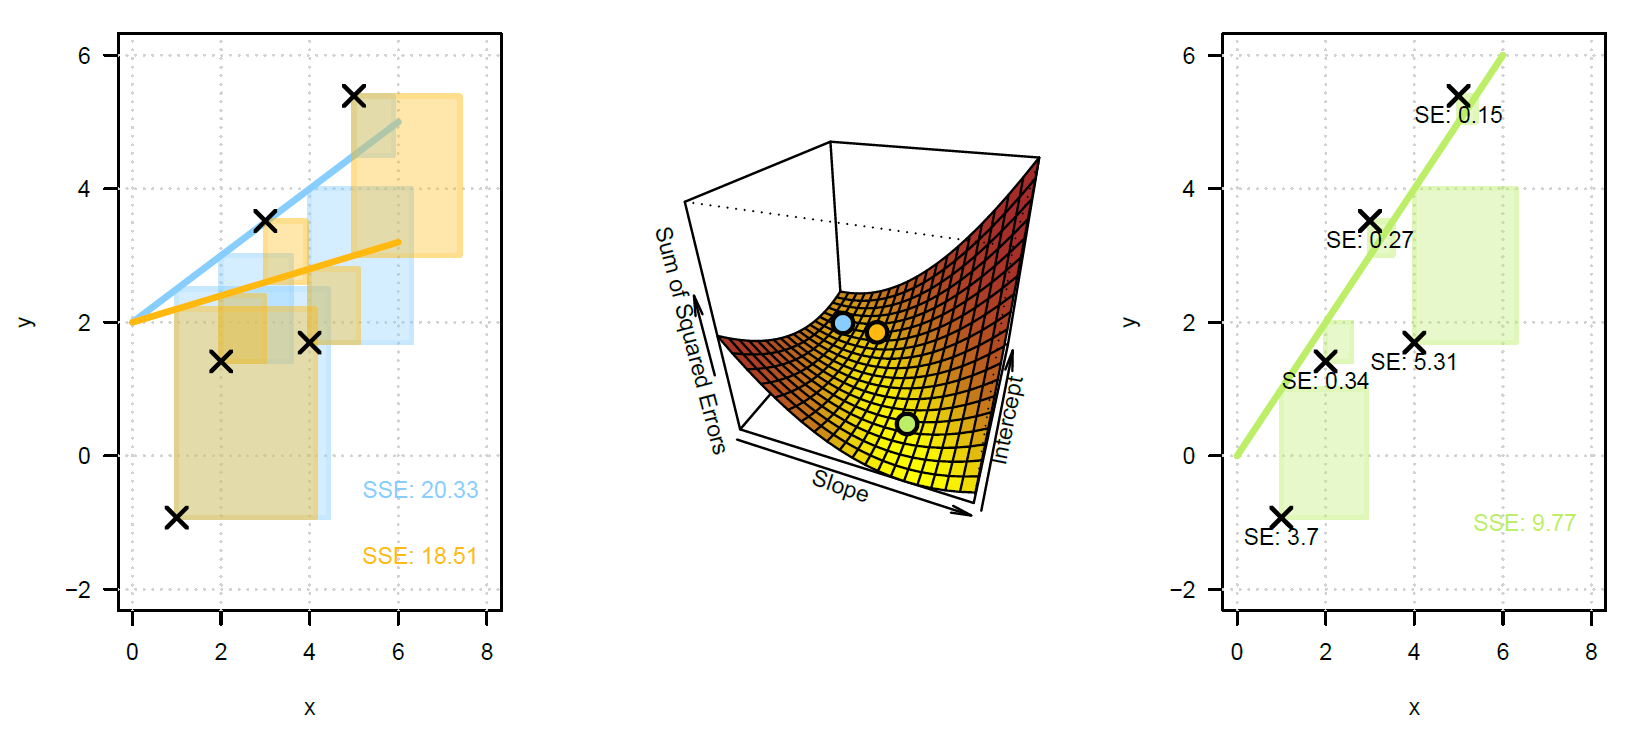
\includegraphics[width=0.9\textwidth]{plots/lin-reg-optim03.png}
\end{center}

\end{vbframe}

%%%%%%%%%%%%%%%%%%%%%%%%%%%%%%%%%%%%%%%%%%%%%%%%%%%%

\begin{frame}{Linear Regression via density estimation}

Let us now assume we want to perform density fitting with a model
$p(\yi|\xi, \theta)$ defined by 
$$
y = 
\theta^T x + \eps = f(x|\theta) + \eps \enspace,
 \text{with  \;\;\;\;}  \eps \sim N\Big(0, \sigma^2\Big)
$$

\pause 

This is a transformation of a normal distributed variable and thus
$$
y \sim N\Big( f(x|\theta), \sigma^2\Big)
$$
and 
$$
 \pdf\Big(y | x , \theta \Big) \propto \exp\Big(-\frac{ (f(x|\theta) - y)^2}{2\sigma^2}\Big)
$$
And the hypothesis space is given by 
$$
 H= \biggl\lbrace
 \pdf\Big(y | x , \theta \Big) | \theta ) \in \mathbb{R}^{p+1} \biggr\rbrace
$$

\end{frame}


\begin{frame}{Linear Regression via density estimation}

The likelihood of the model is given by

$$
\LLt = \prod_{i=1}^n   \pdf\Big(\yi | \xi , \theta \Big)
\propto \exp(-\frac{\sumin (\fxit - \yi)^2}{2\sigma^2})
$$
\pause

The log-likelihood is given by 
$$
\llt \propto \sumin (\fxit - \yi)^2 
$$
and thus log-liklihood maximization is equivalent to our loss minmization approach
$$
\argmax_{\theta}\llt = \argmin_{\theta}\ \sumin (\fxit - \yi)^2 
$$
\end{frame}


\begin{frame}{Example: Linear Regr. With L1 vs L2 Loss}

We could also minimize the L1 loss. This changes the evaluation and
optimization step: \[
\risket = \sumin \Lxyit = \sumin |\yi - \theta^T \xi| \qquad \textsf{(Evaluation)}
\] Much harder to optimize, but the model is less sensitive to outliers.

\scriptsize

\begin{center}
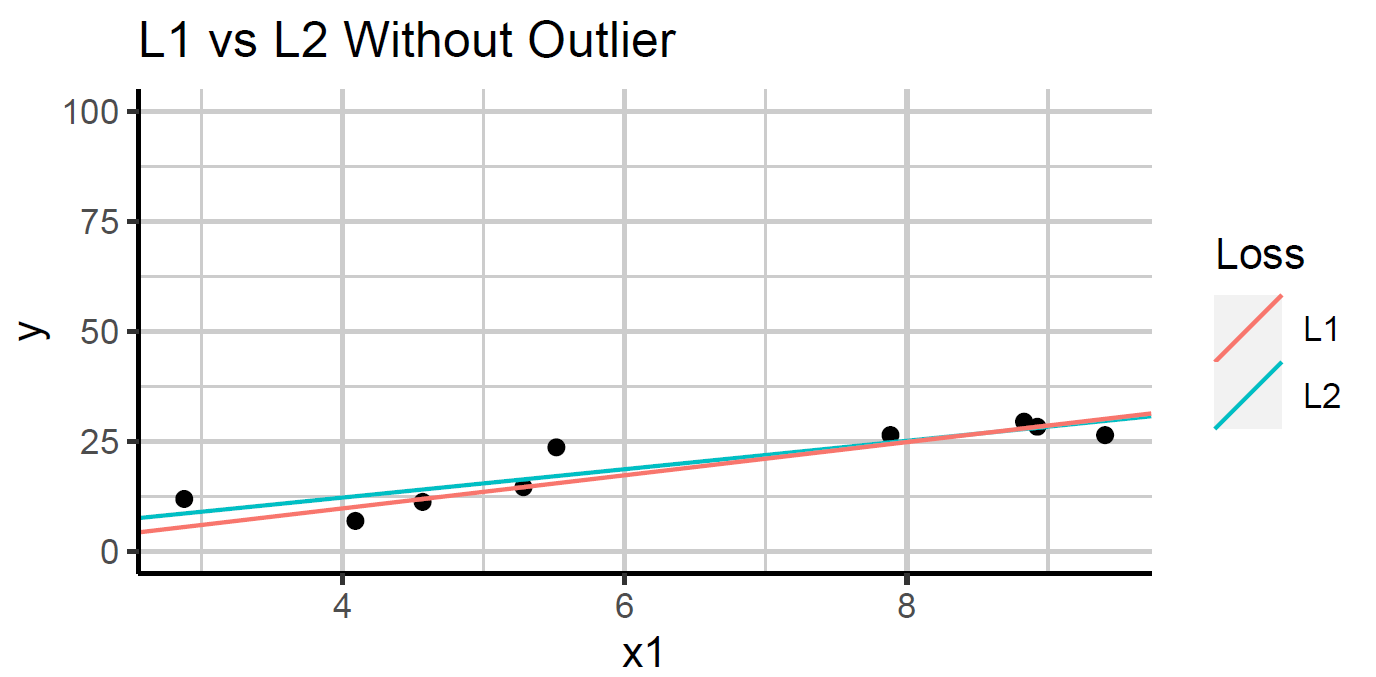
\includegraphics[width=0.7\textwidth]{plots/lin-reg-L1.png}
\end{center}

\normalsize 

\end{frame}

\begin{frame}{Example: Linear Regr. With L1 vs L2 Loss}

Adding an outlier (highlighted red) pulls the line fitted with L2 into
the direction of the outlier:

\scriptsize
\begin{center}
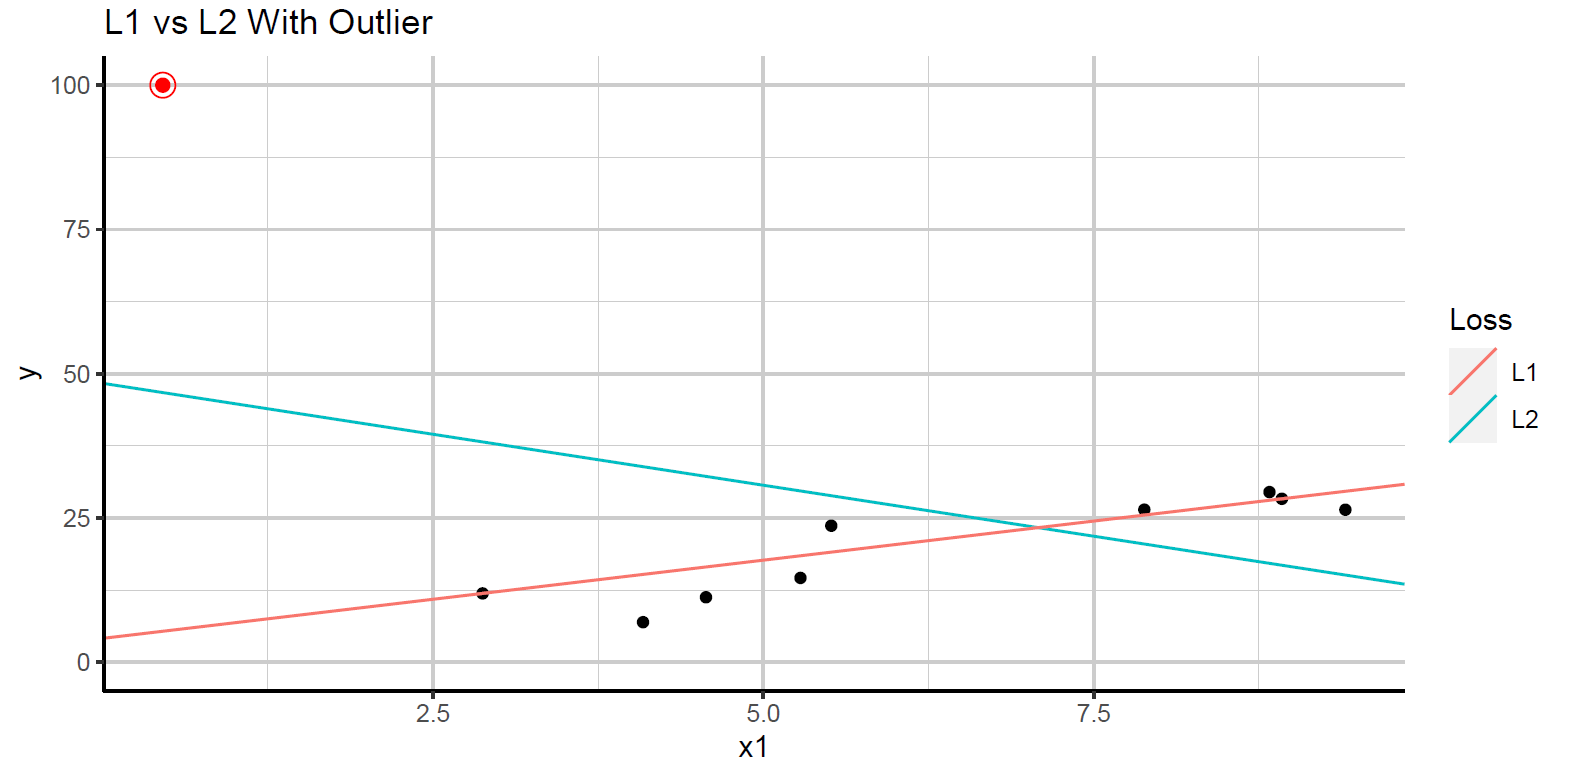
\includegraphics[width=0.8\textwidth]{plots/example-lin-reg.png}
\end{center}

\normalsize 

\end{frame}

%%%%%%%%%%%%%%%%%%%%%%%%%%%%%%%%%%%%%%%%%%%%%%%%%%%%%%%%%

\section{Classification}

\begin{frame}{Binary Classification Task}

\begin{itemize}
\item
  \(y\) is a categorical variable (with two values)
\item
  E.g., sick/healthy, or credit/no credit
\item
  \textbf{Goal}: Predict a class (or membership probabilities)
\end{itemize}

\scriptsize
\begin{center}
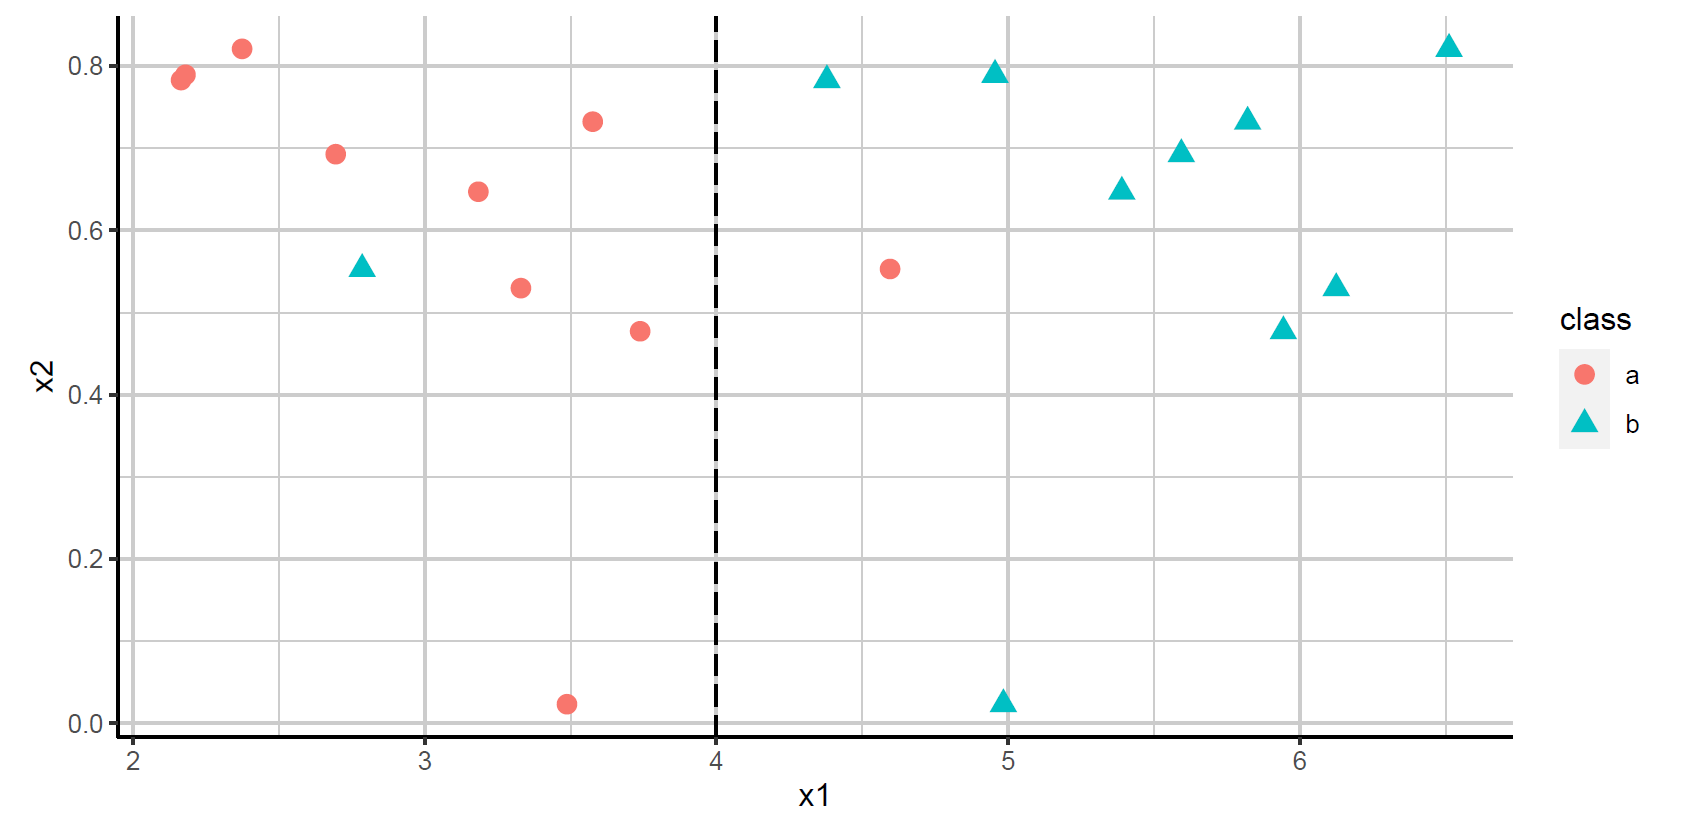
\includegraphics[width=0.8\textwidth]{plots/binary-class.png}
\end{center}

\normalsize 
\end{frame}

%%%%%%%%%%%%%%%%%%%%%%%%%%%%%%%%%%%%%%

\begin{frame}{Linear classification}

Let us assume we have two classes which we encode by $\mathcal{Y}=\{-1,1\}$.
\begin{itemize}

\item Hypothesis space:
we build an affine \textbf{linear classifier}
$$
f(x | \theta)=
\begin{cases}
1 & \text{ for } \theta^T x \ge 0 \\
-1 & \text{ otherwise}
\end{cases}
$$
where we again assume that the intercept $\theta_{0}$ in included in $\theta$.
\pause 

\item Evaluation:
we can measure the training error by the \textbf{Hinge loss}
\begin{equation*}
\Lxyt =\max\{0, 1 - y f(x | \theta) \}
\end{equation*}
\pause

\item Optimization: the resulting minimization problem 
can not be solved analytically. But we will learn about optimizing techniques that can do it.

\end{itemize}
\end{frame}
%%%%%%%%%%%%%%%%%%%%%%%%%%%%%%%%%%%%%%%%%%%%

\begin{frame} {Types of boundaries that can be learned}
  \begin{itemize}
    \item Different values of $\theta$ map to different linear decision boundaries separating the two classes.
    \vspace{5mm}
    \begin{figure}
    \centering
      \scalebox{1}{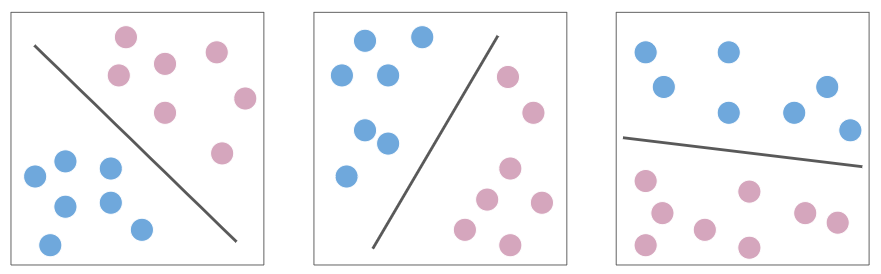
\includegraphics{plots/lin_bound.png}}
  \end{figure}
    \vspace{5mm}
  Note : Only two dimensions pictured here
  \end{itemize}
\end{frame}

\begin{frame} {Types of boundaries that can be learned}
\begin{itemize}
  \item The intercept $\theta_0$, is in ML often (unfortunately) called bias.
  \item It produces an affine shift of the linear decision boundary.
\end{itemize}

\begin{figure}
    \centering
    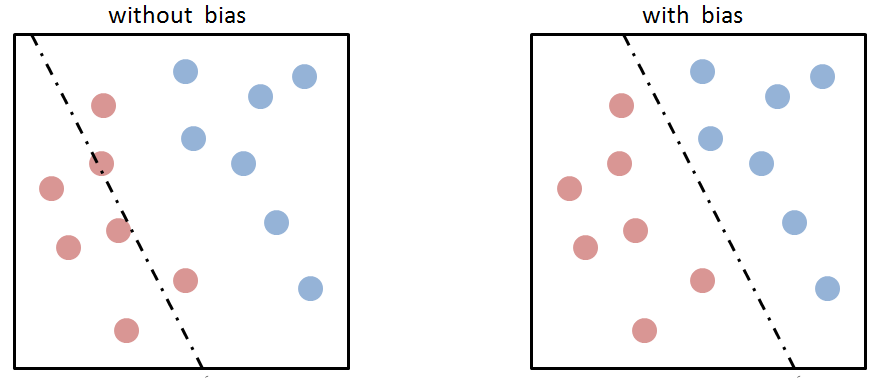
\includegraphics[width=8.5cm]{plots/bias.png}
\end{figure}
\end{frame}

%%%%%%%%%%%%%%%%%%%%%%%%%%%%%%%%%%%%%%%%%%%

\begin{frame}{Classification: Posterior Probabilities}

\begin{itemize}
\item
  Often estimating class probabilities for observations is more
  informative than predicting labels.
\item
  Posterior probabilities are the probability of a class \(k\) occuring,
  given the feature \(x\) \[
  P(Y = k | x)
  \]
\item
  Class estimation for \(x\) via \(\argmax_{k}    P(Y = k | x) \) - just take most
  likely class.
\end{itemize}

\end{frame}

\begin{frame}{Classification: Decision Boundary}

\begin{itemize}
\item
  Area in feature space where there is no unique best class with maximum
  posterior probability, e.g., for binary classification
  \(   P(Y = 1 | x)=   P(Y = 2 | x) \)
\item
  Separates areas in which a specific class is estimated / chosen.
\end{itemize}

\scriptsize
\begin{center}
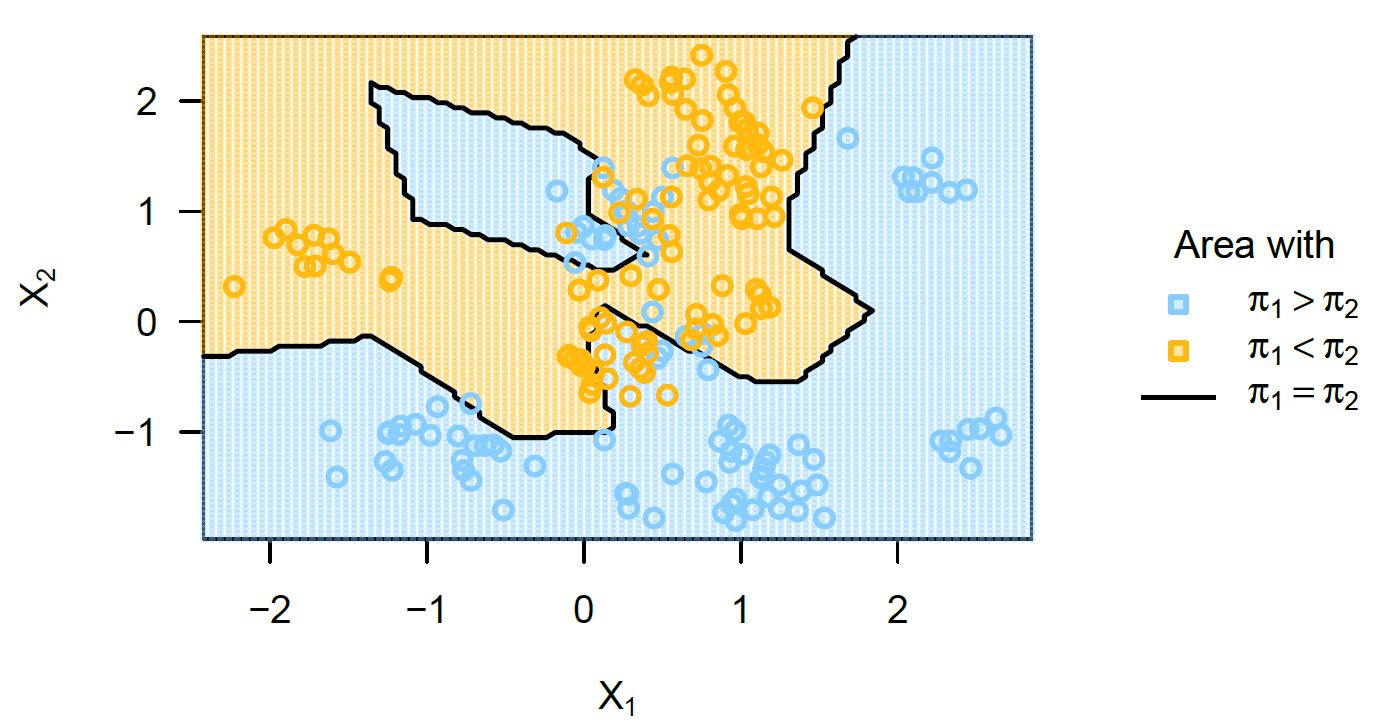
\includegraphics[width=0.8\textwidth]{plots/decision-boundary.png}
\end{center}

\normalsize 

\end{frame}

%%%%%%%%%%%%%%%%%%%%%%%%%%%%%%%%%%%%%%%%%%%%%%%%%

\begin{frame}{Sigmoid/Logistic function}

 
The \emph{logistic function} (often referred to as \emph{sigmoid}) is a bounded, differentiable, real-valued function $\tau: \R \to (0,1)$, $t \to \frac{\exp(t)}{1+\exp(t)}=\frac{1}{{1+\exp(-t)}}$.
\lz

Properties of logistic function:
\begin{itemize}
\item $\lim_{t \to\ -\infty} \tau(t) = 0$ and  $\lim_{t \to \infty} \tau(t) = 1$
\item $\tau(t)$ is symmetrical about the point $(0, 1/2)$
\end{itemize}

\begin{center}
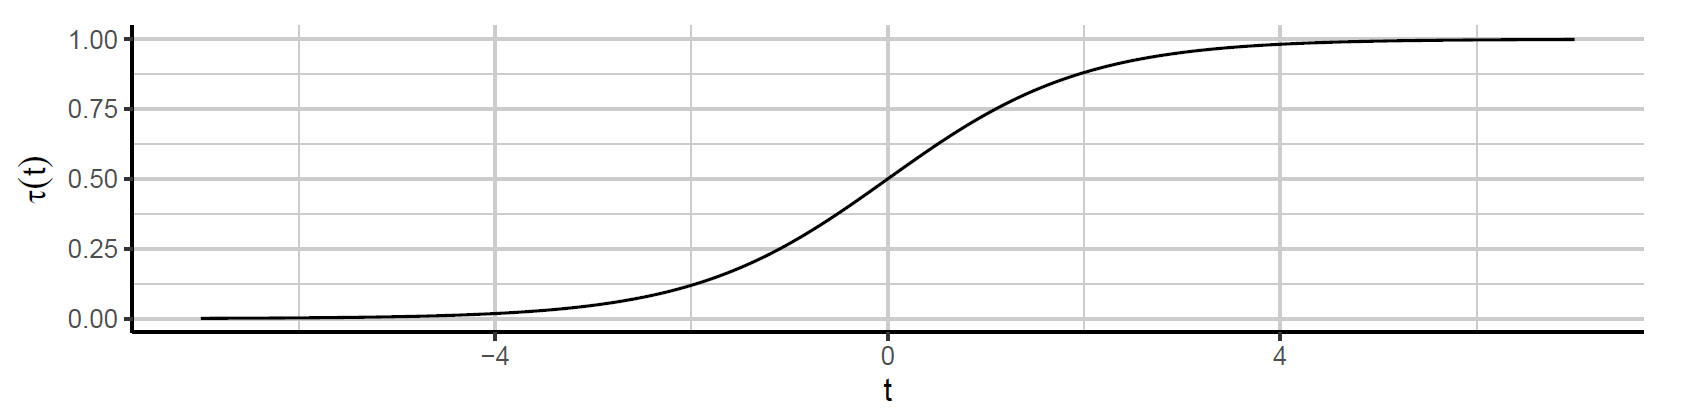
\includegraphics[width=0.9\textwidth]{plots/sigmoid.png}
\end{center}

\end{frame}

%%%%%%%%%%%%%%%%%%%%%%%%%%%%%%%%%%%%%%%%%%%%%%%%%%%%%%

\begin{vbframe}{Logistic regression}

An approach for directly modeling the posterior probabilities of the classes is \textbf{logistic regression}. We will first look at the binary case $y \in \mathcal{Y}=\{0, 1\}$ and define our model as

$$
 P(y = 1 | x, \theta)= \frac{\exp(\theta^Tx)}{1+\exp(\theta^Tx)} = \tau(\theta^T x)
$$


\lz

The logistic function $\tau(t) = \frac{\exp(t)}{1 + \exp(t)}$
transforms the scores 
$\theta^Tx$ into a probability.

\framebreak

\lz

To predicted class labels we predict $y=1$, iff

$$
 P(y = 1 | x, \theta) = \frac{\exp(\theta^T x)}{1+\exp(\theta^Tx)} \ge 0.5,
$$

which is equal to
$$
\theta^T x \ge 0.
$$

So logistic regression gives us a linear classifier:
$$
f(x| \theta) =
=\begin{cases}
1 & \text{ for } x^T\theta \ge 0 \\
0 & \text{ otherwise}
\end{cases}
$$


\framebreak

Logistic regression is usually evaluated based on the \textbf{(log-)likelihood}.

\vspace{-0.2cm}
\small
\begin{align*}
\LLt &= \prod_{i=1}^n P(y = y^{(i)} | x^{(i)}, \theta) \\
 &= \prod_{i=1}^n  P(y = 1 | x^{(i)}, \theta)^{y^{(i)}}[1 - P(y = 1 | x^{(i)}, \theta)]^{1 - y^{(i)}} \\
&= \prod_{i=1}^n  \tau(\theta^T x)^{y^{(i)}} [1 -  \tau(\theta^T x)]^{1 - y^{(i)}}.\\
\end{align*}

\vspace{-0.5cm}
\small
\begin{align*}
\llt &= \sum_{i=1}^n \yi \log[ P(y = 1 | x^{(i)}, \theta)^{y^{(i)}}] + (1-\yi) \log [1 - P(y = 1 | x^{(i)}, \theta)^{y^{(i)}}]\\
\end{align*}

\vspace{-0.3cm}
The negative of the terms of the sum  is also known as \textbf{cross-entropy loss}.
We can minimize it by optimization techniques we will learn about.

\framebreak

%%%%%%%%%%%%%%%%%%%%%%%%%%%%%%%%%%%%%%%%%%%%%%%
\begin{figure}
  \centering
  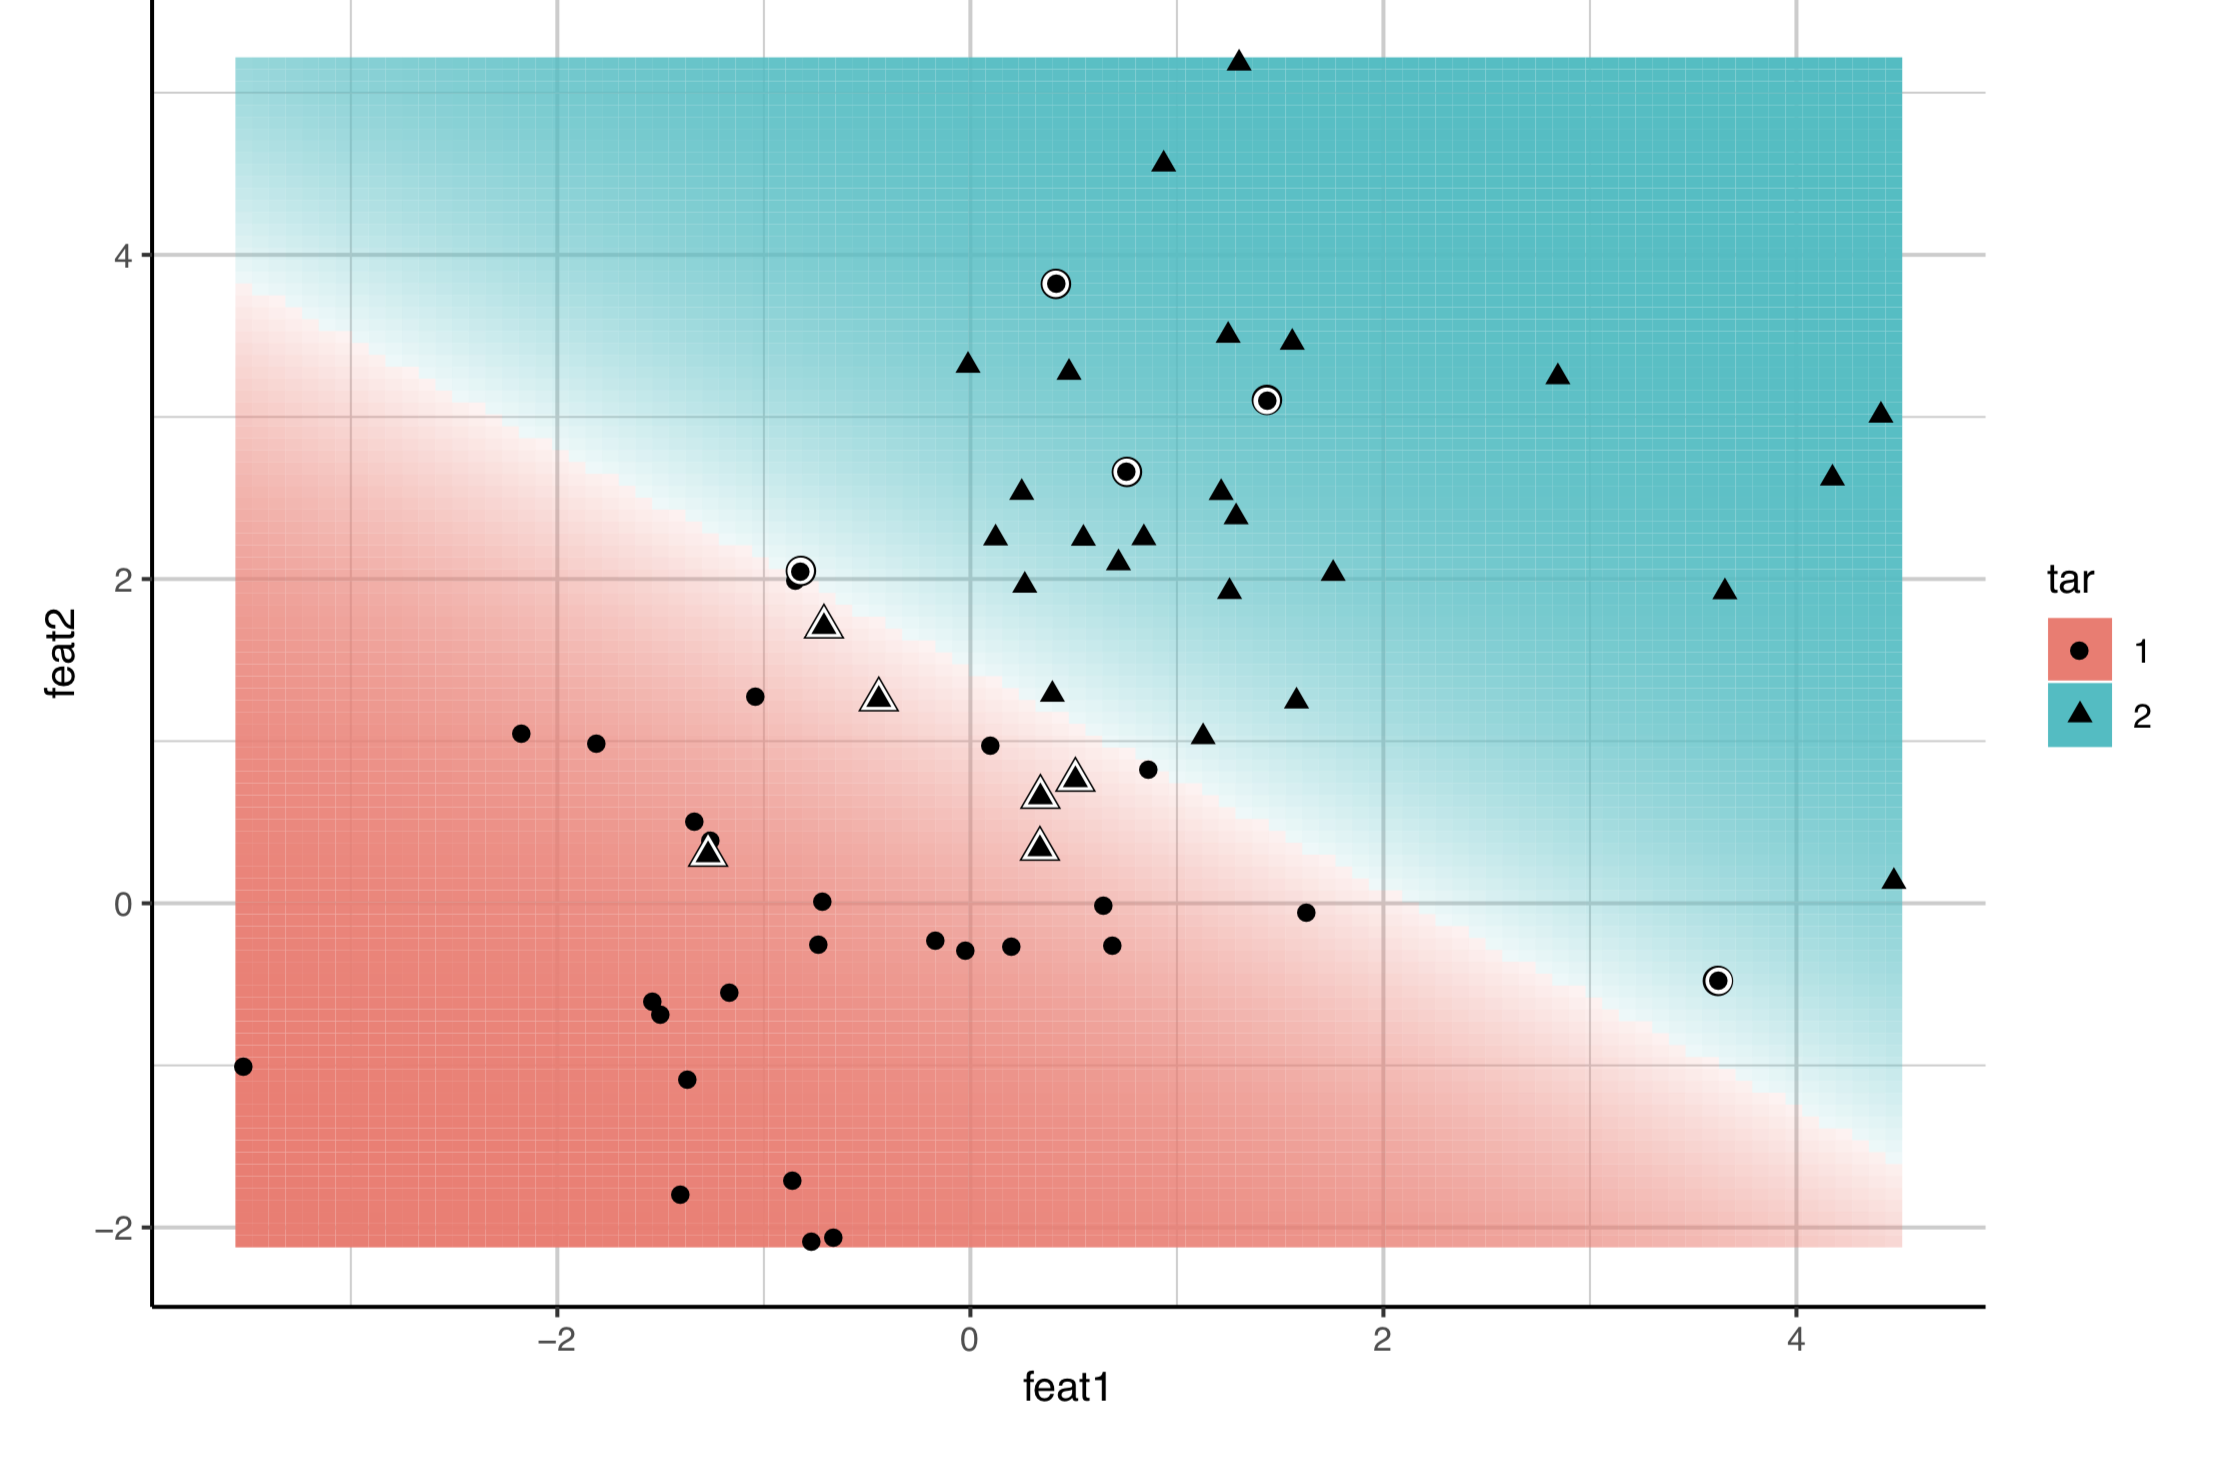
\includegraphics[width=10cm]{plots/LR.png}
\end{figure}

\end{vbframe}

%%%%%%%%%%%%%%%%%%%%%%%%%%%%%%%%%%%%%%%%%

\begin{vbframe}{Generalization to arbitraty score-functions}

In logistic regression, the logistic function transforms 
$y = \theta^Tx$ into a probability:
$\tau(y) = \frac{\exp(y)}{1 + \exp(-y)}$.\\
\lz
The above approach can be generalized: any score-generating model $\fx$ can be turned into probability estimator by using $\tau(f(x))$.

\begin{itemize}
\item $f$ could be another model that outputs a score
\item $\tau$ could be another sigmoid-function (e.g. the cdf of the standard normal distribution which leads to the \emph{probit}-model)
\item an appropriate loss is needed, e.g.
the cross-entropy loss.
One (older) approach is to simply use $\tau(f(x))$ as the model and then minimize the squared loss between $\yh$ and the $(0,1)$ labels.
\end{itemize}
\end{vbframe}
%%%%%%%%%%%%%%%%%%%%%%%%%%%%%%%%%%%%%%%%%%%

\begin{vbframe}{Likelihood and losses}

Let us generalize what we have observed from the comparison between the maximum-likelihood
and the loss-based approach to linear/logistic regression.

The maximum-likelihood principle is to maximize
$$ \LLt = \prod_{i=1}^n \pdfyigxit $$
or to minimize the neg. log-likelihood:
$$ -\llt = -\sumin \lpdfyigxit $$
Now let us define a new loss as:
$$ \Lxyt = - \lpdfygxt $$
And consider the empirical risk
$$\risket = \sumin \Lxyt$$

\begin{itemize}
\item The maximum-likelihood estimator $\thetah$, which we obtain by maximizing $\LLt$ is identical
to the loss-minimal $\thetah$ we obtain by minimizing $\risket$.
\item This implies that we can identify for every 
$\pdfygxt$ an
equivalent loss function which leads to the same point estimator for the parameter vector $\theta$.
\item The other way around does not always work: We cannot identify for every loss function and associated
pdf for the distribution. 
\end{itemize}

\end{vbframe}

%%%%%%%%%%%%%%%%%%%%%%%%%%%%%%%%%%%%%%%%%%

\begin{frame}{Multiclass Classification Task}

\begin{itemize}
\item \(y\) is a categorical variable with \textgreater{} 2 unordered values
\item Each instance belongs to only one class
\item \textbf{Goal}: Predict a class (or membership probabilities)
\end{itemize}

\begin{center}
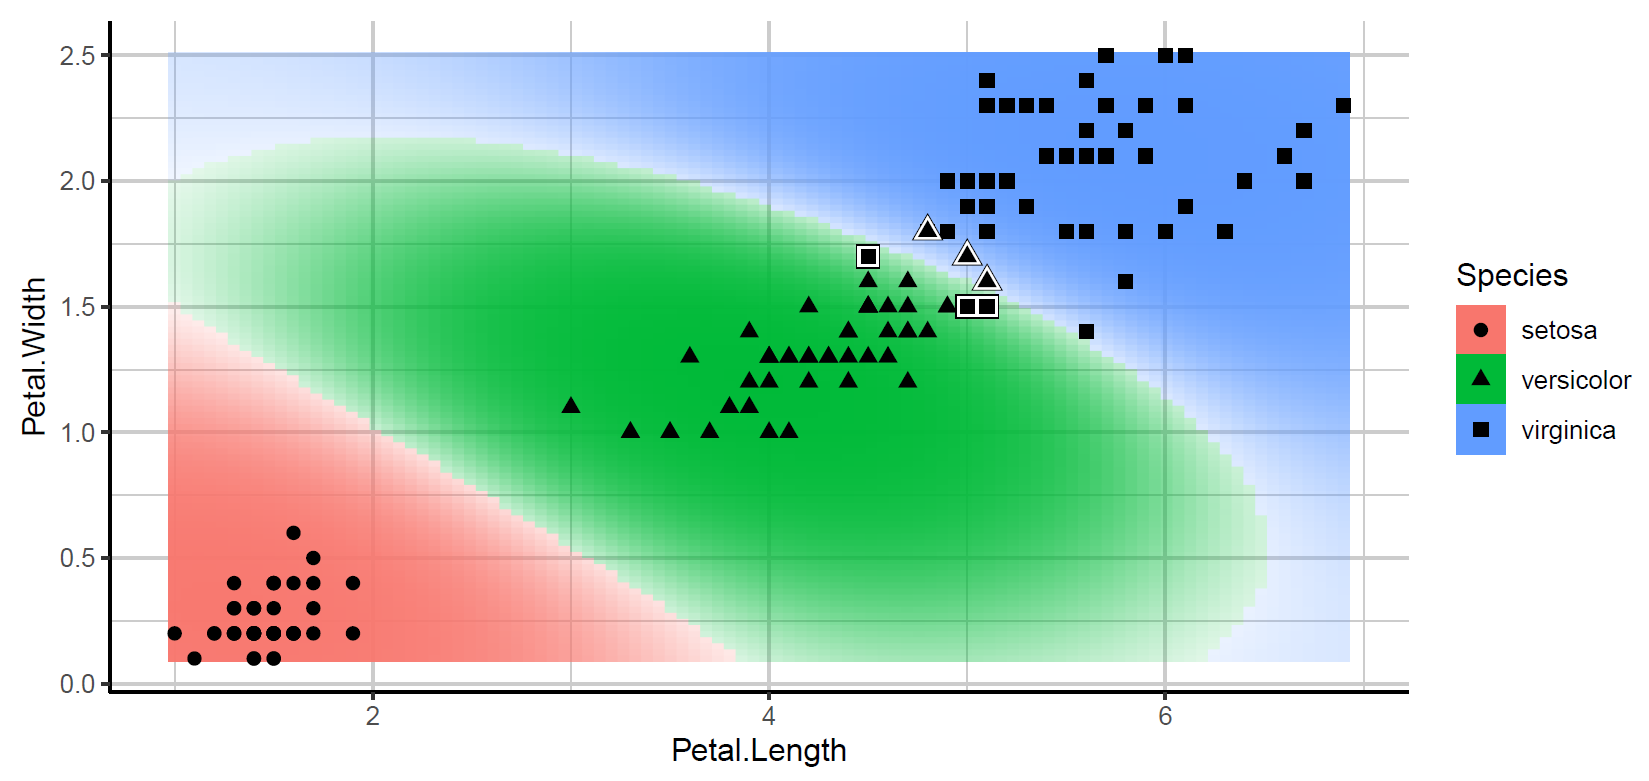
\includegraphics[width=0.8\textwidth]{plots/multi-class.png}
\end{center}

\end{frame}

%%%%%%%%%%%%%%%%%%%%%%%%%%%%%%%%%%%%%%%%%%

\begin{vbframe}{Multinomial Regression and Softmax}

For a categorical response variable $y \in \gset$ with $g>2$ the model extends to

$$
P(y = k | x) = \frac{\exp(\theta_k^Tx)}{\sum_{j=1}^g\exp(\theta_j^Tx)}.
$$
with class specific paramter vectors $\theta_j$

The latter function is called the \textbf{softmax}, and defined on a numerical vector $z$ as
$$
s(z)_k= \frac{\exp(z_k)}{\sum_{j}\exp(z_j)}
$$

\begin{itemize}
\item It is a generalization of the logistic function (check for g=2). \item It \enquote{squashes} a g-dim. real-valued vector $z$ to a vector of the same dimension,
with every entry in the range [0, 1] and all entries adding up to 1.
\end{itemize}
\framebreak

By comparing the posterior probabilities of two categories $k$ and $l$ we end up in a linear function (in $x$),

$$
\log\frac{\pi_k(x)}{\pi_l(x)} = (\theta_k-\theta_l)^Tx.
$$
Again we can employ maximum likelihood based optimization.

\end{vbframe}

%%%%%%%%%%%%%%%%%%%%%%%%%%%%%%%%%%%%%%%%%%%%%

\begin{frame}{Generalization to arbitrary score functions}

This approach can be extended in exactly the same fashion  to other score based models.
For each class $k$ we define a score model $f_k(x)$ (that replaces $\theta_k^Tx$) with parameter vector $\theta_k$.
We then combine these models through the softmax function

$$
P(y=k|x) = \pikx = s(f_1(x), \ldots, f_g(x))_k
$$

and optimize all parameter vectors 
jointly via maximum likelihood

$$
\LLt = \prodin \prodkg \pikxt^{[y = k]}
$$

Negative log-likelihood turns this into empirical risk minimization:

$$
\risket = \sumin \sumkg 1_{[y = k]} \log 
s(f_1(x | \theta_k), \ldots, f_g(x | \theta_g))_k
$$
\end{frame}


\begin{frame}{Summary}
\begin{itemize}
\item The supervised learning scenario is based on labeld training data, a model and a learning algorithm
\item The learning algorithm can be be decomposed into hypothesis space, evaluation, and optimization
\item Evaluation is based on a loss function and  the (empirical) risk
\item Optimization corresponds to empirical risk minimization
\item Linear/logistic regression are examples of regression/classification models 
\item Squared error/cross entropy are examples of loss functions for regression/classification 
\item Likelihood maximization is the standard principle for learning the parameters of probabilitic models (i.e. the loss is the negative log-likelihood)
\item Principles can be generalized from linear models to arbitraty score functions (like neural networks)
\end{itemize}
\end{frame}


\endlecture
\end{document}